% Extended CCIS working manuscript: original study retained, extensions appended.
% Revised explanations and completed payload campaign evidence, 14 November 2026.
\documentclass[runningheads]{llncs}
\usepackage[T1]{fontenc}
\usepackage{amsmath}
\usepackage{newtxtext}
\usepackage[varvw]{newtxmath}
\usepackage{graphicx}
\usepackage{xcolor}
\usepackage{booktabs}
\usepackage{tabularx}
\usepackage{array}
\usepackage{xurl}
\usepackage{listings}
\usepackage[linesnumbered,ruled,vlined]{algorithm2e}
\usepackage{tikz}
\usepackage{pgfplots}
\pgfplotsset{compat=1.17}
\usetikzlibrary{patterns,positioning,arrows.meta}
\usepackage[hidelinks]{hyperref}
\urlstyle{same}
% Class 2.25 provides this command; the fallback keeps class 2.24 compilable.
\providecommand{\Description}[1]{}
\lstdefinestyle{zonecode}{
  basicstyle=\scriptsize\ttfamily,
  breaklines=true,breakatwhitespace=false,
  columns=fullflexible,keepspaces=true,
  frame=single,rulecolor=\color{black},
  keywordstyle=\bfseries,commentstyle=\itshape,
  stringstyle=\ttfamily,showstringspaces=false,
  captionpos=t,aboveskip=\medskipamount,belowskip=\medskipamount
}
\lstset{style=zonecode}
\AtBeginDocument{\renewcommand{\thelstlisting}{\arabic{lstlisting}}}
\setlength{\emergencystretch}{2em}


\newcolumntype{Y}{>{\raggedright\arraybackslash}X}
\definecolor{draftblue}{RGB}{24,73,114}
\newif\ifworkingdraft
\workingdrafttrue
\newcommand{\draftnote}[1]{\ifworkingdraft\par\smallskip\noindent
 {\color{draftblue}\small\textbf{Draft note.} #1}\par\smallskip\fi}
\newcommand{\pending}{\textit{pending}}
\newcommand{\dev}{\textit{in development}}

\begin{document}
\title{Zone: Code--Data Identification, LLM-Assisted Transformation, and Assembly Wrapping for Binary Rewriting}
\titlerunning{Zone: An Extended bin2bin Metamorphic Engine}
\author{Stefano~Bistarelli\orcidID{0000-0001-7411-9678} \and
Jacopo~Di~Benedetto \and
Francesco~Santini\orcidID{0000-0002-3935-4696}}
\authorrunning{S. Bistarelli et al.}
\institute{Dipartimento di Matematica e Informatica, Universit\`a degli Studi di Perugia,\\
Via Vanvitelli 1, 06123 Perugia (PG), Italy\\
\email{stefano.bistarelli@unipg.it}\\
\email{jacopo.dibenedetto@studenti.unipg.it}\\
\email{francesco.santini@unipg.it}}
\maketitle


\begin{abstract}
Rewriting a raw binary requires distinguishing instructions from embedded
data and preserving their references when the layout changes. Zone is a
binary-to-binary metamorphic engine for compact Windows x86 and x64
payloads. This extended study adds symbolic/heuristic and LLM-based data
identification, LLM-proposed instruction transformations, and integration
of assembly wrapping, an existing technique that gives stored bytes
different static and executed instruction interpretations. Six annotated
benign programs are identified exactly in 18 LLM and six symbolic runs.
On 13 separate benign fixtures, LLM transformation yields correct
output buffers in 167/168 x64 and 138/144 x86 invocations. On a separate recovery cohort of 13 previously problematic x64
payloads, working rate improves from 1.2\% to 80.2\%; the corresponding
x86 subset improves from 14.9\% to 25.9\%. In the completed campaigns
on all 102 original payloads,
wrapping constructs 243/306 variants, with 170 passing the functional
harness; LLM transformation constructs 350 outputs across 816 conditions,
with 275 passing. Current raw-file scans give a mean engine detection rate of 0\%
for 207 distinct wrapping outputs and 5.06\% across 322 nonempty reports
for LLM-transformed outputs. Together, the experiments demonstrate improved functional reliability
and evaluate the added transformation modes through construction, execution,
and static detection measurements.
\keywords{Binary Rewriting \and Metamorphic Code \and
Code--Data Identification \and Large Language Models \and Functional Preservation}
\end{abstract}
\section{Introduction}\label{sec:introduction}
Metamorphic rewriting changes a program's instruction sequence, whereas
polymorphic encoding typically changes an encrypted body and its decoding
routine. Both complicate byte-pattern recognition, but expose different
representations during execution~\cite{PEsurveybible,metamorphic1,metamorphic2}.
Zone is a modular \emph{bin2bin} engine for studying these effects on
Windows x86 and x64 payloads without source code or debugging symbols.

\paragraph{Motivation and Contributions of the Extension.}
In this article, we extend our SECRYPT 2026 paper~\cite{zone_secrypt_2026},
which introduced Zone and evaluated 102 payloads under 15 transformation
configurations. The original study identified limits in functional reliability.
One cause is embedded data: a disassembler can interpret a string as
instructions, which rewriting then modifies. Preserving the bytes also
requires maintaining their references when the layout changes. We address
these issues and extend the transformation and evaluation framework with:
\begin{itemize}
\item Alternative symbolic/heuristic and LLM data classifiers, followed by
shared handling of supported data and references
(Section~\ref{sec:code_data}).
\item An LLM transformation path for EQ, NOP, BCF, and IBP, with zero-shot
and two-shot prompting (Section~\ref{sec:llm}).
\item Integration and assessment of the existing assembly-wrapping
technique on x64 and x86 (Section~\ref{sec:wrapping}).
\item New experiments on annotated programs, controlled functional
programs, and the original corpus, including recovery tests, static
detection, output diversity, and cost
(Sections~\ref{sec:methodology} and~\ref{sec:extended_results}).
\end{itemize}

The original architecture, PII design, experiments, and comparison with
Shikata Ga Nai provide the baseline. Reused figures, tables, listings, and
the algorithm carry source citations; added methods and measurements are
identified separately. The selected x64 recovery cohort improves from
1.2\% to 80.2\% working rate, motivating a joint assessment of construction
and execution rather than detection alone.

\paragraph{Scope and terminology.}\label{par:study_scope}
Throughout this article, \emph{working} means that a transformed output
passes the specified functional test. Rate denominators distinguish
planned cases from constructed binaries (Section~\ref{sec:methodology}).
The scope remains compact, position-independent payloads. Full Portable
Executable (PE) rewriting requires additional treatment of imports,
sections, relocations, alignment, and entry points, and signatures may
also occur outside code~\cite{sigdetPEnoncode}. Raw-file scan results and
payload-level execution tests therefore describe the tested representations,
not complete malicious applications or deployed endpoint protection.

Sections~\ref{sec:background}--\ref{sec:comparison} summarize the baseline
methods, results, and limitations. Sections~\ref{sec:code_data}--\ref{sec:wrapping}
present the added methods; Sections~\ref{sec:methodology} and~\ref{sec:extended_results}
describe their evaluation. Section~\ref{sect:related_work} positions the
contributions within prior research, and Section~\ref{sec:conclusion3}
discusses the findings and outlines future research directions.

\section{Background}\label{sec:background}

\subsection{Metamorphic Engines}\label{sub:meth}
A metamorphic engine changes instructions while aiming to preserve
control flow, references, and relevant processor
state~\cite{historycodeobf,identifyingmeth,metworm}. Its rewritten body
executes directly. Polymorphic encoding instead uses a decoding stage:
Shikata Ga Nai varies its stub, but recurring features may remain
recognizable~\cite{sgnstrong}, and decoding can expose the original body
to memory analysis~\cite{codeExtraction}.

\subsection{Morphing Techniques}
The baseline considers EQ, NOP insertion, IBP, and BCF, separately and in
selected combinations. They change instruction vocabulary, add operations,
rearrange blocks, or introduce branches and unreachable regions.
PII additionally separates placement from logical execution order
(Section~\ref{sec:pii}). The following summarizes the original
design~\cite{zone_secrypt_2026}; Section~\ref{sect:related_work} discusses
its antecedents.

\paragraph{Equal Code Substitution.}
EQ replaces an operation with an alternative representation, such as
\texttt{XOR rax, rax} and \texttt{MOV rax, 0x0}. Equivalent effects on one
register do not imply preservation of all processor state.
Table~\ref{tab:instruction_substitutions_x86} reproduces the original
substitution examples, including arithmetic and stack-based sequences.
This transformation family has a long
history~\cite{desai2008towards,desai2010highly,szor2001hunting}.

\begin{table}[t]
    \caption{Instruction substitutions and corresponding encodings (x86). Reproduced from Table~1 of~\cite{zone_secrypt_2026}.}
    \label{tab:instruction_substitutions_x86}
    \small
    \centering
    \setlength{\tabcolsep}{3pt}
    \begin{tabular}{llcl}
        \hline
        \textbf{Original Inst.} & \textbf{Morphed Inst.} & \textbf{Orig. Bytes} & \textbf{Morphed Bytes} \\ \hline
        \texttt{XOR eax, eax} & \texttt{MOV eax, 0} & \texttt{31 C0} & \texttt{B8 00 00 00 00} \\
        \texttt{SUB eax, 1} & \texttt{ADD eax, -1} & \texttt{83 E8 01} & \texttt{83 C0 FF} \\
        \texttt{ADD eax, 2} & \texttt{SUB eax, -2} & \texttt{83 C0 02} & \texttt{83 E8 FE} \\
        \texttt{MOV eax, 0} & \texttt{PUSH 0; POP eax} & \texttt{C7 C0 00..} & \texttt{6A 00 58} \\ \hline
    \end{tabular}
\end{table}

\paragraph{NOP/Dead Code Insertion.}
Inserted operations are intended to leave the relevant computation
unchanged. Table~\ref{tab:nop_instructions} lists the original examples.
Arithmetic no-ops can still affect processor flags; the original
implementation therefore used the flag-preserving sequence in
Table~\ref{tab:flag_preserving_nop}. Such repeated sequences may themselves
become recognizable artifacts~\cite{pushfmeth}.

\begin{table}[t]
    \caption{NOP-like operations and their encodings. Reproduced from Table~2 of~\cite{zone_secrypt_2026}.}
    \label{tab:nop_instructions}
    \small
    \centering
    \setlength{\tabcolsep}{3pt}
    \begin{tabular}{ll}
        \hline
        \textbf{Example} & \textbf{Compiled Opcode} \\ \hline
        \verb|NOP| & \verb|0x90| \\ \hline
        \verb|SUB rax, 0x0| & \verb|0x48, 0x83, 0xE8, 0x00| \\ \hline
        \verb|ADD rax, 0x0| & \verb|0x48, 0x83, 0xC0, 0x00| \\ \hline
        \verb|MOV rax, rax| & \verb|0x48, 0x89, 0xC0| \\ \hline
        \verb|LEA rax, [rax + 0]| & \verb|0x48, 0x8D, 0x40, 0x00| \\ \hline
        \verb|PUSH rax; POP rax| & \verb|0x50, 0x58| \\ \hline
        \verb|OR rax, rax| & \verb|0x48, 0x09, 0xC0| \\ \hline
        \verb|XOR rax, 0x0| & \verb|0x48, 0x83, 0xF0, 0x00| \\ \hline
        \verb|AND rax, rax| & \verb|0x48, 0x21, 0xC0| \\ \hline
        \verb|INC rax; DEC rax| & \verb|0x48, 0xFF, 0xC0; 0x48, 0xFF, 0xC8| \\ \hline
        \verb|DEC rax; INC rax| & \verb|0x48, 0xFF, 0xC8; 0x48, 0xFF, 0xC0| \\ \hline
        \verb|SAR rax, 0x0| & \verb|0x48, 0xC1, 0xF8, 0x00| \\ \hline
        \verb|SHR rax, 0x0| & \verb|0x48, 0xC1, 0xE8, 0x00| \\ \hline
        \verb|SHL rax, 0x0| & \verb|0x48, 0xC1, 0xE0, 0x00| \\ \hline
        \verb|RCL rax, 0x0| & \verb|0x48, 0xC1, 0xD0, 0x00| \\ \hline
        \verb|RCR rax, 0x0| & \verb|0x48, 0xC1, 0xD8, 0x00| \\ \hline
    \end{tabular}
\end{table}

\begin{table}[htbp]
    \centering
    \caption{Flag-preserving insertion example. Reproduced from Table~3 of~\cite{zone_secrypt_2026}.}
    \label{tab:flag_preserving_nop}
    \small
    \centering
    \setlength{\tabcolsep}{3pt}
    \begin{tabular}{ll}
        \hline
        \textbf{Instruction}    & \textbf{Compiled Opcode} \\ \hline
        \verb|PUSHF|             & \verb|0x9C|                \\ \hline
        \verb|ADD rax, 0x0|      & \verb|0x48, 0x83, 0xC0, 0x00| \\ \hline
        \verb|POPF|              & \verb|0x9D|                \\ \hline
    \end{tabular}
\end{table}

\paragraph{Instruction Block Permutation.}
IBP divides instructions into blocks, links each block to its logical
successor, permutes their placement while retaining the entry block, and
updates control-flow targets. The chosen granularity affects layout
variation and overhead. Instructions within a block can remain unchanged,
so rearrangement need not alter short internal patterns.

\paragraph{Bogus Control Flow.}
BCF adds branches around code that is not intended to execute. The implementation uses conditions with predetermined outcomes to exclude the inserted region from the execution path~\cite{bin2binobf,llvmobf}. Table~\ref{table:bcf_code} reproduces the illustrative block from the conference article: the condition transfers control past the padding at addresses \texttt{0x11}--\texttt{0x17}.

\begin{table}[t]
\caption{Illustrative BCF block. Reproduced from Table~4 of~\cite{zone_secrypt_2026}.}
\small
\centering
\setlength{\tabcolsep}{3pt}
\label{table:bcf_code}
\begin{tabular}{ll}
    \hline
    \textbf{Address}    & \textbf{Instruction} \\ \hline

    \verb|0x0|  & 	\verb|mov rax, 0x1|  \\ \hline
    \verb|0x7|	&   \verb|cmp rax, 0x1|  \\ \hline
    \verb|0xb| 	&   \verb|je 0x18|  \\ \hline
    \verb|0x11|	&   \verb|nop|  \\ \hline
    \verb|0x12|	&   \verb|nop|  \\ \hline
    \verb|0x13|	&   \verb|nop|  \\ \hline
    \verb|0x14|	&   \verb|nop|  \\ \hline
    \verb|0x15|	&   \verb|nop|  \\ \hline
    \verb|0x16|	&   \verb|nop|  \\ \hline
    \verb|0x17|	&   \verb|nop|  \\ \hline
    \verb|0x18|	&\verb|original code.......|    \\ \hline
\end{tabular}
\end{table}


\section{Zone Architecture}\label{sec:developing_meth}
Zone is implemented in Python: Capstone disassembles the input, the
selected transformations modify its instruction representation, and
Keystone assembles the output. This \emph{bin2bin} interface requires
neither source code nor Program Database (PDB) symbols. Although initial
development also explored PE files, the evaluated scope remains raw
payloads~\cite{zone_secrypt_2026}. The public repository is linked in the
Data and Artifact Availability statement.

\subsection{Position-Independent Instruction}\label{sec:pii}
PII was introduced in the conference paper~\cite{zone_secrypt_2026}. It decouples the physical position of an instruction from its place in the intended execution sequence.

\paragraph{Organization.}
Consider an instruction such as \texttt{ADD rax, 1}. In the PII representation it is placed in a wrapper rather than relying on adjacency to its successor. The wrapper executes the original operation and transfers control to a redirector. An offset table supplies the location of the next logical instruction. Figure~\ref{fig:pii_layout} reproduces the overall layout, while the listings below document the components of the original design.

\begin{figure}[t]
\centering
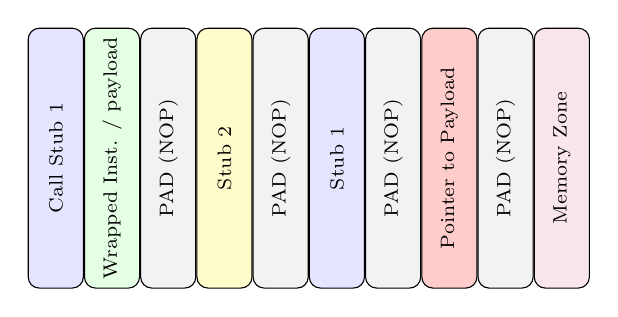
\begin{tikzpicture}[
    font=\scriptsize,
    node distance=0.0cm,
    every node/.style={
        rotate=90,
        minimum width=3.3cm,
        minimum height=0.7cm,
        text centered,
        draw,
        fill=gray!10,
        rounded corners,
        inner xsep=2pt,
        inner ysep=6pt
    }
]

\node (stubCall)  [fill=blue!10]    {Call Stub 1};
\node (payload)   [below=of stubCall, fill=green!10]  {Wrapped Inst. / payload};
\node (pad1)      [below=of payload]                  {PAD (NOP)};
\node (stub2)     [below=of pad1, fill=yellow!20]     {Stub 2};
\node (pad2)      [below=of stub2]                    {PAD (NOP)};
\node (stub1)     [below=of pad2, fill=blue!10]       {Stub 1};
\node (pad3)      [below=of stub1]                    {PAD (NOP)};
\node (payloadPtr)[below=of pad3, fill=red!20]        {Pointer to Payload};
\node (pad4)      [below=of payloadPtr]               {PAD (NOP)};
\node (memZone)   [below=of pad4, fill=purple!10]     {Memory Zone};

\end{tikzpicture}
\Description{A schematic separates the initial call, instruction wrappers, redirector components, padding, offset information, and memory region.}
\caption{PII payload layout. Adapted from Fig.~1 of~\cite{zone_secrypt_2026}.}
\label{fig:pii_layout}
\end{figure}

The representation has four components: a base-address stub (Stub1), a
redirector (Stub2), an offset table, and wrapped instructions.
Stub1 establishes the runtime location (Listing~\ref{lst:stub1}).
Each wrapper executes its original instruction and supplies its logical
index to Stub2 (Listing~\ref{lst:instrWrap}). The redirector uses the base
address and offset table to locate the successor, preserving the state
it uses before transferring control (Listing~\ref{lst:stub2red}).

\paragraph{Physical Placement.}
The original implementation permutes complete wrappers, treating each five-instruction wrapper as a unit. The offset table is updated for the resulting placement. Execution still starts with the initial call to Stub1; logical succession is represented by the table rather than by the wrappers' physical adjacency.

\begin{lstlisting}[label={lst:stub1},language={[x86masm]Assembler}, basicstyle=\scriptsize\ttfamily, caption={Base-address component. Reproduced from Listing~1 of~\cite{zone_secrypt_2026}.}]
pop <random_unused_reg>;    popping 2nd instruction address
mov [<random_unused_reg> - 5 + <init_address>],  <random_unused_reg>; move it to a memory slot
push <random_unused_reg>; push just to avoid altering the stack
jmp <random_unused_reg>; return to the caller (2nd instruction)
\end{lstlisting}

\begin{lstlisting}[label={lst:instrWrap}, language={[x86masm]Assembler}, basicstyle=\scriptsize\ttfamily, caption={Instruction wrapper. Reproduced from Listing~2 of~\cite{zone_secrypt_2026}.}]
pop rax;                    ; popping rax because we just used it to save jmp address
lea rsp, [rsp + 8];         ; adjusting stack to avoid stack overflow
ORIGINAL_INSTRUCTION;       ; original instruction
push <0x3e8 + counter>;     ; pushing instruction original index + a constant
jmp <stub2_address>;        ; Jumping to 'redirector' stub 
\end{lstlisting}

\noindent\begin{minipage}{\linewidth}
\begin{lstlisting}[label={lst:stub2red},language={[x86masm]Assembler}, basicstyle=\scriptsize\ttfamily, caption={x64 redirector. Reproduced from Listing~3 of~\cite{zone_secrypt_2026}.}]
push rax;                                       saving original 'rax' register state
push rcx;                                       saving original 'rcx' register state
mov rcx, [rsp + 0x10] ;                         getting the instruction index from the stack.
pushf;                                          saving original CPU flags
sub rcx, 0x3e8; ;                               subtracting a constant to get instr index
inc rcx;                                        increase instruction number
mov rax, [rip + init_addr_offset];              get payload base address
mov rcx, [rax + mem_address - 5 + rcx * 8];     get next instruction address
sub rcx, 0x5;                                   just because base address is 2nd instruction
add rax, rcx;                                   add payload base address to the offset
popf;                                           restore cpu flags
pop rcx;                                        restore rcx value
jmp rax;                                        jmp to next instruction
\end{lstlisting}

\end{minipage}

\paragraph{Architectural Variants.}
Listings~\ref{lst:stub2red} and~\ref{lst:stub286} show the published x64 and x86 redirectors. In addition to the different register widths, they differ in how the required address is obtained: the x86 version uses the call-based mechanism documented in the original listing rather than x64 RIP-relative addressing.

\begin{lstlisting}[label={lst:stub286},language={[x86masm]Assembler}, basicstyle=\scriptsize\ttfamily, caption={x86 redirector. Reproduced from Listing~4 of~\cite{zone_secrypt_2026}.}]
push eax;
push ecx;
mov ecx, [esp + 0x8]
pushf;
sub ecx, 0x3e8;
inc ecx;

call <stub2_address + 0x14>;    calling pop eax, 0x14 is pop eax offset from stub2 address
pop eax;                        popping eax puts in eax the value of the instruction pointer

mov eax, [eax + <init_addr_offset>];
mov ecx, [eax + <mem_address> - 5 + ecx * 4];
sub ecx, 0x5
add eax, ecx
popf;
pop ecx;
jmp eax;
\end{lstlisting}

\subsection{How Instructions Are Patched}\label{sec:instr_patch}
Moving instructions can invalidate their references. Patching updates
tracked control-flow destinations and other supported references for
the modified layout. Algorithm~\ref{alg:zonealg} reproduces the original
workflow~\cite{zone_secrypt_2026}, within the scope defined in
Section~\ref{sec:introduction}.

\begin{algorithm}[t]

\caption{High-level Zone workflow. Reproduced from Algorithm~1 of~\cite{zone_secrypt_2026}.}\label{alg:zonealg}

\scriptsize

\SetKwProg{Fn}{Function}{}{}
\SetKwFor{ForEach}{for each}{}{end}
\SetKwIF{If}{ElseIf}{Else}{if}{}{else if}{else}{end}

\KwData{raw\_bytes}
\KwResult{Transformed binary}

\textbf{global} instruction\_list $\gets$ []\;
\textbf{global} instruction\_dict $\gets$ \{\}\;
\textbf{global} label\_table $\gets$ []\;

\BlankLine

\Fn{\textbf{disass} \label{fun:disas} }{

    CAPSTONE.SKIPDATA $\gets$ TRUE\;\label{fun:skipdata}

    \ForEach{instruction in disasm(raw\_bytes)}{
        instruction\_list.append(instruction)\;
        instruction\_dict[instruction.address] $\gets$ instruction\;

        \If{instruction is X86.Control\_flow\_instruction}{
            jump\_address $\gets$ extract\_address(instruction.op\_string)\;
            label\_table.append((instruction, instruction\_dict[jump\_address]))\;
        }
    }
}

\BlankLine

\Fn{\textbf{update\_instructions} \label{fun:update_instr}}{
    new\_instruction\_dict $\gets$ \{\}\;

    \ForEach{instruction in instruction\_list}{
        address $\gets$ instruction.previous\_instruction.address + len(instruction.previous\_instruction.bytes)\;
        instruction.address $\gets$ address\;

        new\_instruction\_dict[instruction.address] $\gets$ instruction\;
    }

    instruction\_dict $\gets$ new\_instruction\_dict\;
}

\BlankLine

\Fn{\textbf{morph} \label{fun:morph}} {
    equal\_code\_substitution()\;
    nop\_insertion()\;
    instruction\_block\_shuffling()\;
    bogus\_control\_flow()\;
    position\_independent\_instruction()\;
}

\BlankLine

\Fn{\textbf{adjust\_label\_table} \label{fun:adj_lab_tab}}{
    update\_instructions()\;

    \ForEach{entry in label\_table}{
        jmp\_addr $\gets$ extract\_address(entry[0].op\_string)\;
        jmp\_addr\_new $\gets$ entry[1].address\;

        new\_instruction $\gets$ keystone.assemble(
        ``entry[0].mnemonic jmp\_addr\_new'')\;

        entry[0] $\gets$ new\_instruction\;
    }
}

\BlankLine

\Fn{\textbf{main}}{
    disass()\;
    morph()\;
    adjust\_label\_table()\;
    write\_to\_file()\; \label{fun:writefile}
}

\end{algorithm}

\subsection{Transformation Pipeline}
Algorithm~\ref{alg:zonealg} first constructs instruction objects and an
address-indexed lookup. A label table associates tracked branches with
target objects, retaining those associations as addresses change.
Capstone's \texttt{Skipdata} option does not resolve inline data that also
decodes as instructions~\cite{bin2binobf}. After transformation, addresses
are recomputed, tracked branches are reassembled against updated targets,
and the resulting bytes are written to a raw binary. The added preparation
and transformation paths are described in
Sections~\ref{sec:code_data}--\ref{sec:wrapping}.

\section{Published Experimental Baseline}\label{sec:results}


This section summarizes the conference study~\cite{zone_secrypt_2026}.
Figure~\ref{fig:all_payloads} reaggregates its retained scan records with
corrected configuration labels; no new scans are included. VirusTotal scans supplied verdicts from more than 70 engines, subject to the file-format limitations discussed below.

The corpus comprises 38 x64 and 64 x86 Windows payloads, mostly from
Metasploit, including reverse and bind shells. It represents selected
payload types rather than all Windows malware; large DLL-based components
are outside scope. Architecture comparisons also reflect the different
input memberships.

\paragraph{Testing Method.}
Each of the fifteen configurations was applied to every input, with ten generated variants per input and configuration to expose variation in the transformation process. The five individual transformations and ten combinations were:

\begin{itemize}
    \item \textbf{Single:} NOP (\texttt{nop}), Equal Code Substitution (\texttt{eq}), Bogus Control Flow (\texttt{bcf}), Instruction Block Permutation (\texttt{ibp}), and Position-Independent Instruction (\texttt{pii}).
    \item \textbf{Combined:} \texttt{eq\_nop\_bcf}, \texttt{eq\_nop\_ibp}, \texttt{eq\_nop\_pii}, \texttt{eq\_nop}, \texttt{eq\_bcf}, \texttt{eq\_ibp}, \texttt{eq\_pii}, \texttt{nop\_bcf}, \texttt{nop\_ibp} and \texttt{nop\_pii}.
\end{itemize}

The \emph{detection rate} for an individual file is the fraction of scanning engines that returned a malicious verdict; summaries aggregate these per-file measurements. Figure~\ref{fig:all_payloads} reports a reanalysis of 15,020 distinct
file paths from 15,021 saved records, retaining the latest record for the
repeated path. Each file uses its recorded engine-response denominator. The corresponding baseline averages for the original files were 21.67\% for x64 and 22.63\% for x86.

\begin{figure}[tbp]
\centering
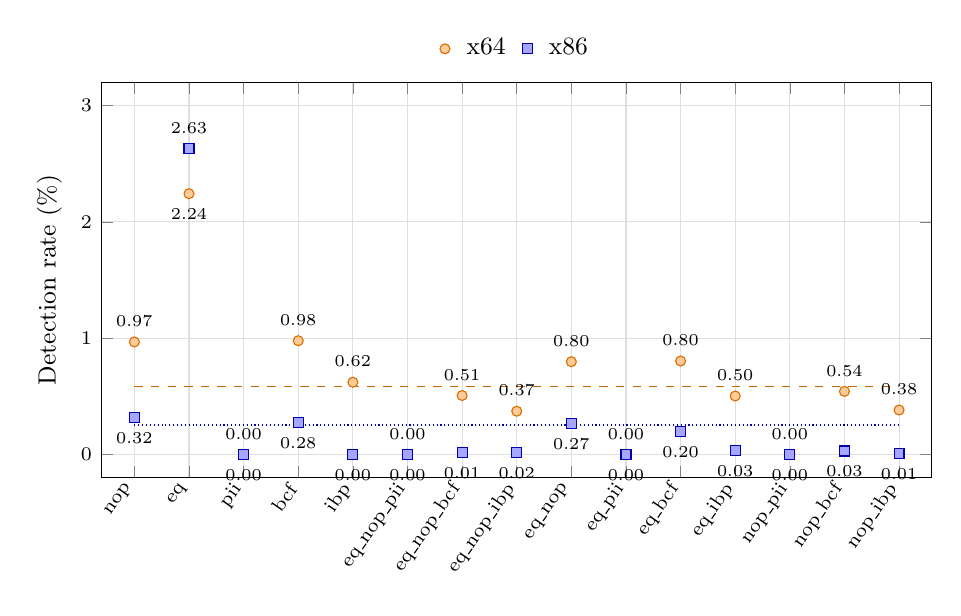
\begin{tikzpicture}
\begin{axis}[
width=\linewidth,height=6.6cm,
ylabel={Detection rate (\%)},ymin=-0.2,ymax=3.2,xmin=-0.6,xmax=14.6,
xtick={0,...,14},
xticklabels={nop,eq,pii,bcf,ibp,eq\_nop\_pii,eq\_nop\_bcf,eq\_nop\_ibp,eq\_nop,eq\_pii,eq\_bcf,eq\_ibp,nop\_pii,nop\_bcf,nop\_ibp},
xticklabel style={rotate=55,anchor=east,font=\scriptsize},
yticklabel style={font=\scriptsize},label style={font=\small},
grid=major,grid style={gray!25},scaled y ticks=false,
legend style={at={(0.5,1.03)},anchor=south,legend columns=2,column sep=4pt,font=\small,draw=none},
clip=false,
]
\addplot[orange!80!black,dashed,no marks,forget plot] coordinates {(0,0.580598) (14,0.580598)};
\addplot[blue!65!black,densely dotted,no marks,forget plot] coordinates {(0,0.252471) (14,0.252471)};
\addplot[only marks,mark size=1.8pt,orange!85!black,mark=*,mark options={fill=orange!40}] coordinates {(0,0.966990) (1,2.242475) (2,0.000000) (3,0.977516) (4,0.620360) (5,0.000000) (6,0.506048) (7,0.371006) (8,0.796921) (9,0.000000) (10,0.802818) (11,0.502046) (12,0.000000) (13,0.541333) (14,0.381452)};
\addlegendentry{x64}
\node[anchor=south,yshift=2pt,font=\fontsize{6}{7}\selectfont] at (axis cs:0,0.966990) {0.97};
\node[anchor=north,yshift=-2pt,font=\fontsize{6}{7}\selectfont] at (axis cs:1,2.242475) {2.24};
\node[anchor=south,yshift=2pt,font=\fontsize{6}{7}\selectfont] at (axis cs:2,0.000000) {0.00};
\node[anchor=south,yshift=2pt,font=\fontsize{6}{7}\selectfont] at (axis cs:3,0.977516) {0.98};
\node[anchor=south,yshift=2pt,font=\fontsize{6}{7}\selectfont] at (axis cs:4,0.620360) {0.62};
\node[anchor=south,yshift=2pt,font=\fontsize{6}{7}\selectfont] at (axis cs:5,0.000000) {0.00};
\node[anchor=south,yshift=2pt,font=\fontsize{6}{7}\selectfont] at (axis cs:6,0.506048) {0.51};
\node[anchor=south,yshift=2pt,font=\fontsize{6}{7}\selectfont] at (axis cs:7,0.371006) {0.37};
\node[anchor=south,yshift=2pt,font=\fontsize{6}{7}\selectfont] at (axis cs:8,0.796921) {0.80};
\node[anchor=south,yshift=2pt,font=\fontsize{6}{7}\selectfont] at (axis cs:9,0.000000) {0.00};
\node[anchor=south,yshift=2pt,font=\fontsize{6}{7}\selectfont] at (axis cs:10,0.802818) {0.80};
\node[anchor=south,yshift=2pt,font=\fontsize{6}{7}\selectfont] at (axis cs:11,0.502046) {0.50};
\node[anchor=south,yshift=2pt,font=\fontsize{6}{7}\selectfont] at (axis cs:12,0.000000) {0.00};
\node[anchor=south,yshift=2pt,font=\fontsize{6}{7}\selectfont] at (axis cs:13,0.541333) {0.54};
\node[anchor=south,yshift=2pt,font=\fontsize{6}{7}\selectfont] at (axis cs:14,0.381452) {0.38};
\addplot[only marks,mark size=1.8pt,blue!70!black,mark=square*,mark options={fill=blue!35}] coordinates {(0,0.318914) (1,2.628536) (2,0.000000) (3,0.275768) (4,0.000000) (5,0.000000) (6,0.012336) (7,0.016502) (8,0.265433) (9,0.000000) (10,0.199616) (11,0.030866) (12,0.000000) (13,0.028783) (14,0.010307)};
\addlegendentry{x86}
\node[anchor=north,yshift=-2pt,font=\fontsize{6}{7}\selectfont] at (axis cs:0,0.318914) {0.32};
\node[anchor=south,yshift=2pt,font=\fontsize{6}{7}\selectfont] at (axis cs:1,2.628536) {2.63};
\node[anchor=north,yshift=-2pt,font=\fontsize{6}{7}\selectfont] at (axis cs:2,0.000000) {0.00};
\node[anchor=north,yshift=-2pt,font=\fontsize{6}{7}\selectfont] at (axis cs:3,0.275768) {0.28};
\node[anchor=north,yshift=-2pt,font=\fontsize{6}{7}\selectfont] at (axis cs:4,0.000000) {0.00};
\node[anchor=north,yshift=-2pt,font=\fontsize{6}{7}\selectfont] at (axis cs:5,0.000000) {0.00};
\node[anchor=north,yshift=-2pt,font=\fontsize{6}{7}\selectfont] at (axis cs:6,0.012336) {0.01};
\node[anchor=north,yshift=-2pt,font=\fontsize{6}{7}\selectfont] at (axis cs:7,0.016502) {0.02};
\node[anchor=north,yshift=-2pt,font=\fontsize{6}{7}\selectfont] at (axis cs:8,0.265433) {0.27};
\node[anchor=north,yshift=-2pt,font=\fontsize{6}{7}\selectfont] at (axis cs:9,0.000000) {0.00};
\node[anchor=north,yshift=-2pt,font=\fontsize{6}{7}\selectfont] at (axis cs:10,0.199616) {0.20};
\node[anchor=north,yshift=-2pt,font=\fontsize{6}{7}\selectfont] at (axis cs:11,0.030866) {0.03};
\node[anchor=north,yshift=-2pt,font=\fontsize{6}{7}\selectfont] at (axis cs:12,0.000000) {0.00};
\node[anchor=north,yshift=-2pt,font=\fontsize{6}{7}\selectfont] at (axis cs:13,0.028783) {0.03};
\node[anchor=north,yshift=-2pt,font=\fontsize{6}{7}\selectfont] at (axis cs:14,0.010307) {0.01};
\end{axis}
\end{tikzpicture}
\Description{Historical detection rates reaggregated from deduplicated saved records, with configuration labels aligned to their filenames.}
\caption{Reanalysis of the historical raw-file scans of~\cite{zone_secrypt_2026}.
Configuration labels follow the file records; duplicate paths are counted once.
Dashed lines are equal-weight means over the 15 configurations (x64: 0.58\%; x86: 0.25\%).}
\label{fig:all_payloads}
\end{figure}

The plotted observations vary by transformation and architecture. Several configurations involving PII received no malicious verdicts in these raw-file scans, whereas EQ retained more detections. These measurements describe the tested representations and submission conditions; they should be interpreted together with the functional results.

\label{par:working_rate}
The \emph{working rate} is the proportion passing the execution checks:
an expected connection for reverse shells, port opening for bind shells,
or exception-free termination for other generic cases.
Table~\ref{tab:overall_working_update} consolidates historical rates
recomputed from retained test records with the update for 49 retested
inputs. This replaces the earlier working-rate plot and aligns
configuration labels with those records. The historical study reported
greater stability for EQ and lower stability for PII, particularly on x86.



\paragraph{Evaluation Limitations.}
The raw-file comparison follows the scope defined in
Section~\ref{sec:introduction}. Unsupported-format responses and omitted
execution-based analysis affect how these scan results should be
interpreted~\cite{zone_secrypt_2026}; response accounting is detailed in
Section~\ref{sec:methodology}.

\section{Size and Statistical Measurements}\label{sect:var_metrics}
The conference paper measured file length, entropy change, and cosine
similarity to characterize the rewritten representations~\cite{zone_secrypt_2026}.

\paragraph{Payload Length Variation.}
Let $L_i$ denote the byte length of a transformed file and let $n$ be the number of files considered for a configuration. The reported mean length is:
\[
\overline{L} = \frac{1}{n} \sum_{i=1}^{n} L_i
\]

\begin{figure}[tbp]
\centering
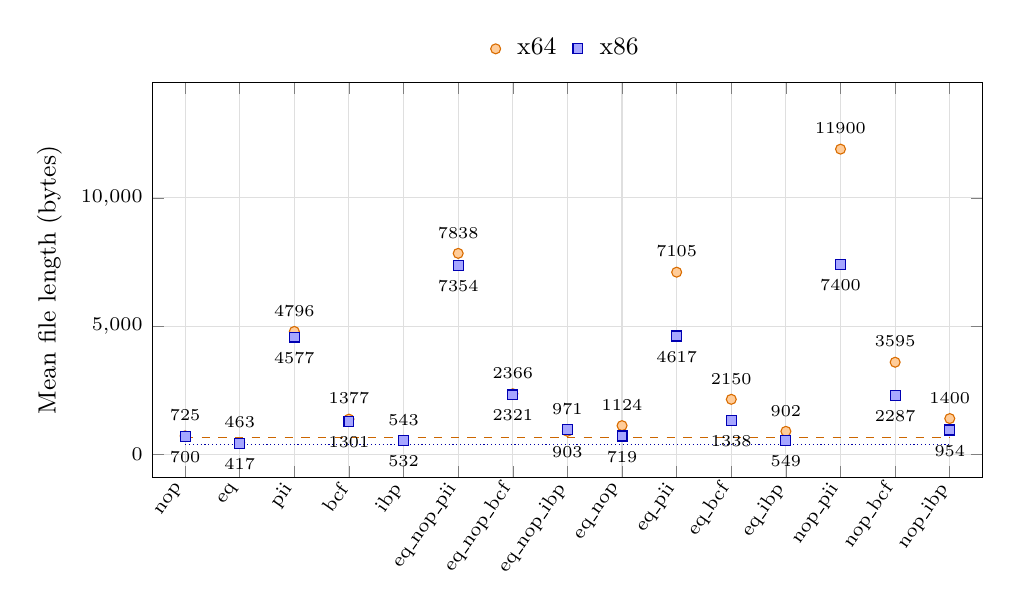
\begin{tikzpicture}
\begin{axis}[
width=\linewidth,height=6.6cm,
ylabel={Mean file length (bytes)},ymin=-900,ymax=14500,xmin=-0.6,xmax=14.6,
xtick={0,...,14},
xticklabels={nop,eq,pii,bcf,ibp,eq\_nop\_pii,eq\_nop\_bcf,eq\_nop\_ibp,eq\_nop,eq\_pii,eq\_bcf,eq\_ibp,nop\_pii,nop\_bcf,nop\_ibp},
xticklabel style={rotate=55,anchor=east,font=\scriptsize},
yticklabel style={font=\scriptsize},label style={font=\small},
grid=major,grid style={gray!25},scaled y ticks=false,
legend style={at={(0.5,1.03)},anchor=south,legend columns=2,column sep=4pt,font=\small,draw=none},
clip=false,
]
\addplot[orange!80!black,dashed,no marks,forget plot] coordinates {(0,652.632) (14,652.632)};
\addplot[blue!65!black,densely dotted,no marks,forget plot] coordinates {(0,400.750) (14,400.750)};
\addplot[only marks,mark size=1.8pt,orange!85!black,mark=*,mark options={fill=orange!40}] coordinates {(0,725) (1,463) (2,4796) (3,1377) (4,543) (5,7838) (6,2366) (7,903) (8,1124) (9,7105) (10,2150) (11,902) (12,11900) (13,3595) (14,1400)};
\addlegendentry{x64}
\node[anchor=south,yshift=2pt,font=\fontsize{6}{7}\selectfont] at (axis cs:0,725) {725};
\node[anchor=south,yshift=2pt,font=\fontsize{6}{7}\selectfont] at (axis cs:1,463) {463};
\node[anchor=south,yshift=2pt,font=\fontsize{6}{7}\selectfont] at (axis cs:2,4796) {4796};
\node[anchor=south,yshift=2pt,font=\fontsize{6}{7}\selectfont] at (axis cs:3,1377) {1377};
\node[anchor=south,yshift=2pt,font=\fontsize{6}{7}\selectfont] at (axis cs:4,543) {543};
\node[anchor=south,yshift=2pt,font=\fontsize{6}{7}\selectfont] at (axis cs:5,7838) {7838};
\node[anchor=south,yshift=2pt,font=\fontsize{6}{7}\selectfont] at (axis cs:6,2366) {2366};
\node[anchor=north,yshift=-2pt,font=\fontsize{6}{7}\selectfont] at (axis cs:7,903) {903};
\node[anchor=south,yshift=2pt,font=\fontsize{6}{7}\selectfont] at (axis cs:8,1124) {1124};
\node[anchor=south,yshift=2pt,font=\fontsize{6}{7}\selectfont] at (axis cs:9,7105) {7105};
\node[anchor=south,yshift=2pt,font=\fontsize{6}{7}\selectfont] at (axis cs:10,2150) {2150};
\node[anchor=south,yshift=2pt,font=\fontsize{6}{7}\selectfont] at (axis cs:11,902) {902};
\node[anchor=south,yshift=2pt,font=\fontsize{6}{7}\selectfont] at (axis cs:12,11900) {11900};
\node[anchor=south,yshift=2pt,font=\fontsize{6}{7}\selectfont] at (axis cs:13,3595) {3595};
\node[anchor=south,yshift=2pt,font=\fontsize{6}{7}\selectfont] at (axis cs:14,1400) {1400};
\addplot[only marks,mark size=1.8pt,blue!70!black,mark=square*,mark options={fill=blue!35}] coordinates {(0,700) (1,417) (2,4577) (3,1301) (4,532) (5,7354) (6,2321) (7,971) (8,719) (9,4617) (10,1338) (11,549) (12,7400) (13,2287) (14,954)};
\addlegendentry{x86}
\node[anchor=north,yshift=-2pt,font=\fontsize{6}{7}\selectfont] at (axis cs:0,700) {700};
\node[anchor=north,yshift=-2pt,font=\fontsize{6}{7}\selectfont] at (axis cs:1,417) {417};
\node[anchor=north,yshift=-2pt,font=\fontsize{6}{7}\selectfont] at (axis cs:2,4577) {4577};
\node[anchor=north,yshift=-2pt,font=\fontsize{6}{7}\selectfont] at (axis cs:3,1301) {1301};
\node[anchor=north,yshift=-2pt,font=\fontsize{6}{7}\selectfont] at (axis cs:4,532) {532};
\node[anchor=north,yshift=-2pt,font=\fontsize{6}{7}\selectfont] at (axis cs:5,7354) {7354};
\node[anchor=north,yshift=-2pt,font=\fontsize{6}{7}\selectfont] at (axis cs:6,2321) {2321};
\node[anchor=south,yshift=2pt,font=\fontsize{6}{7}\selectfont] at (axis cs:7,971) {971};
\node[anchor=north,yshift=-2pt,font=\fontsize{6}{7}\selectfont] at (axis cs:8,719) {719};
\node[anchor=north,yshift=-2pt,font=\fontsize{6}{7}\selectfont] at (axis cs:9,4617) {4617};
\node[anchor=north,yshift=-2pt,font=\fontsize{6}{7}\selectfont] at (axis cs:10,1338) {1338};
\node[anchor=north,yshift=-2pt,font=\fontsize{6}{7}\selectfont] at (axis cs:11,549) {549};
\node[anchor=north,yshift=-2pt,font=\fontsize{6}{7}\selectfont] at (axis cs:12,7400) {7400};
\node[anchor=north,yshift=-2pt,font=\fontsize{6}{7}\selectfont] at (axis cs:13,2287) {2287};
\node[anchor=north,yshift=-2pt,font=\fontsize{6}{7}\selectfont] at (axis cs:14,954) {954};
\end{axis}
\end{tikzpicture}
\Description{Mean transformed-file length. Reference lines indicate the original-file means (x64: 652.632 bytes; x86: 400.750 bytes). Orange circles identify x64 and blue squares identify x86.}
\caption{Mean transformed-file length. Reference lines indicate the original-file means (x64: 652.632 bytes; x86: 400.750 bytes). Data from Fig.~4 of~\cite{zone_secrypt_2026}; redrawn for the present format.}
\label{fig:length_comparison}
\end{figure}

The size results in Figure~\ref{fig:length_comparison} show substantial growth for PII and BCF configurations. Some EQ-containing configurations instead produced smaller average outputs than the original-file reference. The conference paper associated this observation with the implementation's treatment of data during disassembly; the size measurement alone does not establish that any removed bytes were semantically irrelevant.

\paragraph{Delta Entropy.}
The reported entropy change compares the transformed representation, $H_{tech}$, with its original, $H_{orig}$, using the percentage difference:

\begin{equation}
\Delta H \; (\%) = \frac{H_{tech} - H_{orig}}{H_{orig}} \times 100
\end{equation}

The measurements were computed on raw bytes and on tokenized assembly. Figures~\ref{fig:shan_entropy} and~\ref{fig:shan_entropy_bytes} retain the published results. The assembly-based representation also permits comparison with the metrics discussed by Mohseni et al.~\cite{llmobf}.

NOP insertion increased assembly entropy, whereas PII decreased it,
consistent with repeated bookkeeping instructions. BCF combined small
entropy changes with increased length and a changed opcode distribution;
IBP could change layout while retaining similar instruction frequencies.
Entropy describes the representation, not functional preservation.

\begin{figure}[tbp]
\centering
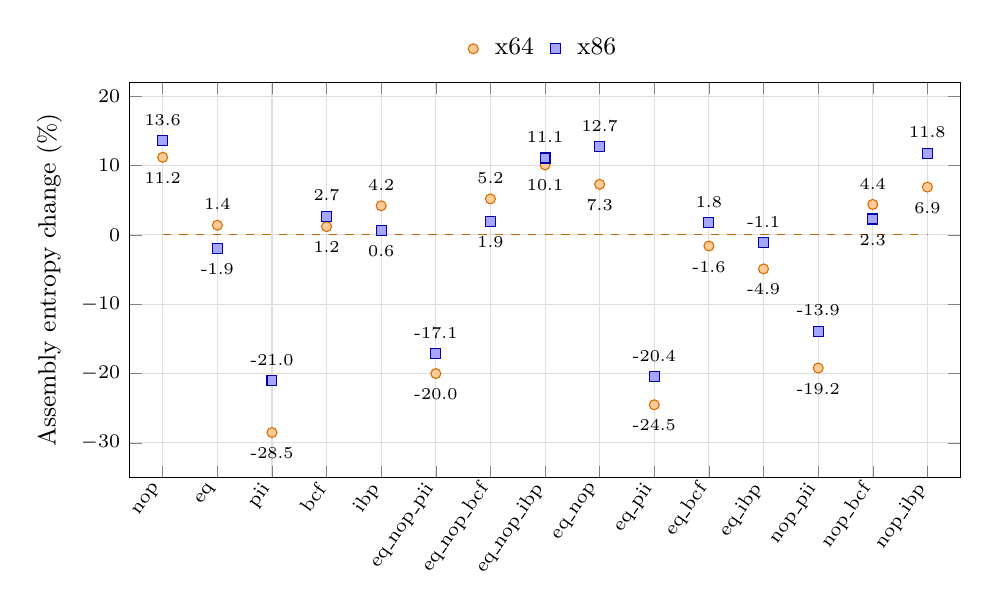
\begin{tikzpicture}
\begin{axis}[
width=\linewidth,height=6.6cm,
ylabel={Assembly entropy change (\%)},ymin=-35,ymax=22,xmin=-0.6,xmax=14.6,
xtick={0,...,14},
xticklabels={nop,eq,pii,bcf,ibp,eq\_nop\_pii,eq\_nop\_bcf,eq\_nop\_ibp,eq\_nop,eq\_pii,eq\_bcf,eq\_ibp,nop\_pii,nop\_bcf,nop\_ibp},
xticklabel style={rotate=55,anchor=east,font=\scriptsize},
yticklabel style={font=\scriptsize},label style={font=\small},
grid=major,grid style={gray!25},scaled y ticks=false,
legend style={at={(0.5,1.03)},anchor=south,legend columns=2,column sep=4pt,font=\small,draw=none},
clip=false,
]
\addplot[orange!80!black,dashed,no marks,forget plot] coordinates {(0,0) (14,0)};
\addplot[only marks,mark size=1.8pt,orange!85!black,mark=*,mark options={fill=orange!40}] coordinates {(0,11.2) (1,1.4) (2,-28.5) (3,1.2) (4,4.2) (5,-20.0) (6,5.2) (7,10.1) (8,7.3) (9,-24.5) (10,-1.6) (11,-4.9) (12,-19.2) (13,4.4) (14,6.9)};
\addlegendentry{x64}
\node[anchor=north,yshift=-2pt,font=\fontsize{6}{7}\selectfont] at (axis cs:0,11.2) {11.2};
\node[anchor=south,yshift=2pt,font=\fontsize{6}{7}\selectfont] at (axis cs:1,1.4) {1.4};
\node[anchor=north,yshift=-2pt,font=\fontsize{6}{7}\selectfont] at (axis cs:2,-28.5) {-28.5};
\node[anchor=north,yshift=-2pt,font=\fontsize{6}{7}\selectfont] at (axis cs:3,1.2) {1.2};
\node[anchor=south,yshift=2pt,font=\fontsize{6}{7}\selectfont] at (axis cs:4,4.2) {4.2};
\node[anchor=north,yshift=-2pt,font=\fontsize{6}{7}\selectfont] at (axis cs:5,-20.0) {-20.0};
\node[anchor=south,yshift=2pt,font=\fontsize{6}{7}\selectfont] at (axis cs:6,5.2) {5.2};
\node[anchor=north,yshift=-2pt,font=\fontsize{6}{7}\selectfont] at (axis cs:7,10.1) {10.1};
\node[anchor=north,yshift=-2pt,font=\fontsize{6}{7}\selectfont] at (axis cs:8,7.3) {7.3};
\node[anchor=north,yshift=-2pt,font=\fontsize{6}{7}\selectfont] at (axis cs:9,-24.5) {-24.5};
\node[anchor=north,yshift=-2pt,font=\fontsize{6}{7}\selectfont] at (axis cs:10,-1.6) {-1.6};
\node[anchor=north,yshift=-2pt,font=\fontsize{6}{7}\selectfont] at (axis cs:11,-4.9) {-4.9};
\node[anchor=north,yshift=-2pt,font=\fontsize{6}{7}\selectfont] at (axis cs:12,-19.2) {-19.2};
\node[anchor=south,yshift=2pt,font=\fontsize{6}{7}\selectfont] at (axis cs:13,4.4) {4.4};
\node[anchor=north,yshift=-2pt,font=\fontsize{6}{7}\selectfont] at (axis cs:14,6.9) {6.9};
\addplot[only marks,mark size=1.8pt,blue!70!black,mark=square*,mark options={fill=blue!35}] coordinates {(0,13.6) (1,-1.9) (2,-21.0) (3,2.7) (4,0.6) (5,-17.1) (6,1.9) (7,11.1) (8,12.7) (9,-20.4) (10,1.8) (11,-1.1) (12,-13.9) (13,2.3) (14,11.8)};
\addlegendentry{x86}
\node[anchor=south,yshift=2pt,font=\fontsize{6}{7}\selectfont] at (axis cs:0,13.6) {13.6};
\node[anchor=north,yshift=-2pt,font=\fontsize{6}{7}\selectfont] at (axis cs:1,-1.9) {-1.9};
\node[anchor=south,yshift=2pt,font=\fontsize{6}{7}\selectfont] at (axis cs:2,-21.0) {-21.0};
\node[anchor=south,yshift=2pt,font=\fontsize{6}{7}\selectfont] at (axis cs:3,2.7) {2.7};
\node[anchor=north,yshift=-2pt,font=\fontsize{6}{7}\selectfont] at (axis cs:4,0.6) {0.6};
\node[anchor=south,yshift=2pt,font=\fontsize{6}{7}\selectfont] at (axis cs:5,-17.1) {-17.1};
\node[anchor=north,yshift=-2pt,font=\fontsize{6}{7}\selectfont] at (axis cs:6,1.9) {1.9};
\node[anchor=south,yshift=2pt,font=\fontsize{6}{7}\selectfont] at (axis cs:7,11.1) {11.1};
\node[anchor=south,yshift=2pt,font=\fontsize{6}{7}\selectfont] at (axis cs:8,12.7) {12.7};
\node[anchor=south,yshift=2pt,font=\fontsize{6}{7}\selectfont] at (axis cs:9,-20.4) {-20.4};
\node[anchor=south,yshift=2pt,font=\fontsize{6}{7}\selectfont] at (axis cs:10,1.8) {1.8};
\node[anchor=south,yshift=2pt,font=\fontsize{6}{7}\selectfont] at (axis cs:11,-1.1) {-1.1};
\node[anchor=south,yshift=2pt,font=\fontsize{6}{7}\selectfont] at (axis cs:12,-13.9) {-13.9};
\node[anchor=north,yshift=-2pt,font=\fontsize{6}{7}\selectfont] at (axis cs:13,2.3) {2.3};
\node[anchor=south,yshift=2pt,font=\fontsize{6}{7}\selectfont] at (axis cs:14,11.8) {11.8};
\end{axis}
\end{tikzpicture}
\Description{Percentage entropy change for tokenized assembly; the reference level is zero. Orange circles identify x64 and blue squares identify x86.}
\caption{Percentage entropy change for tokenized assembly; the reference level is zero. Data from Fig.~5 of~\cite{zone_secrypt_2026}; redrawn for the present format.}
\label{fig:shan_entropy}
\end{figure}

\begin{figure}[tbp]
\centering
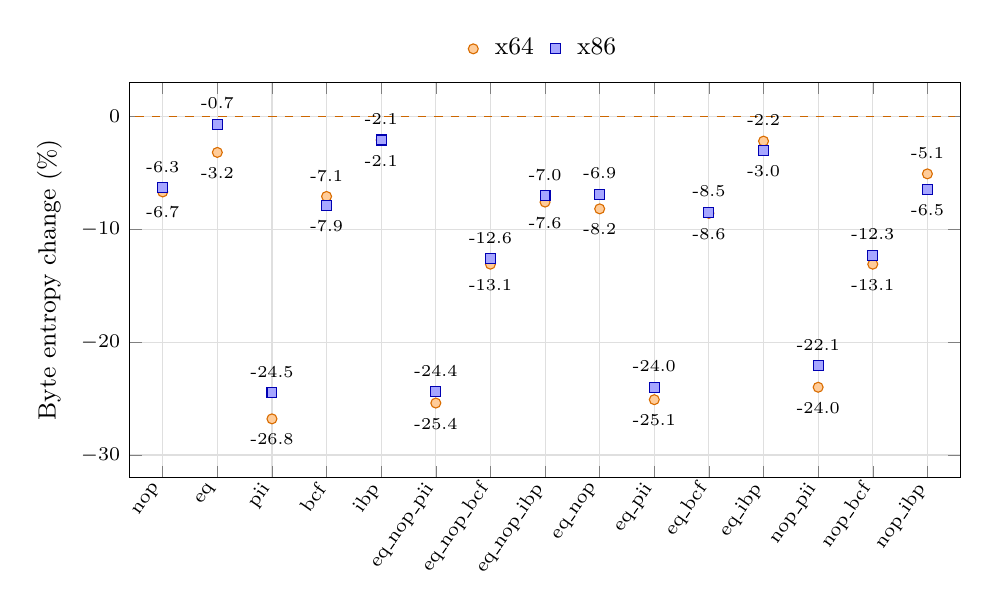
\begin{tikzpicture}
\begin{axis}[
width=\linewidth,height=6.6cm,
ylabel={Byte entropy change (\%)},ymin=-32,ymax=3,xmin=-0.6,xmax=14.6,
xtick={0,...,14},
xticklabels={nop,eq,pii,bcf,ibp,eq\_nop\_pii,eq\_nop\_bcf,eq\_nop\_ibp,eq\_nop,eq\_pii,eq\_bcf,eq\_ibp,nop\_pii,nop\_bcf,nop\_ibp},
xticklabel style={rotate=55,anchor=east,font=\scriptsize},
yticklabel style={font=\scriptsize},label style={font=\small},
grid=major,grid style={gray!25},scaled y ticks=false,
legend style={at={(0.5,1.03)},anchor=south,legend columns=2,column sep=4pt,font=\small,draw=none},
clip=false,
]
\addplot[orange!80!black,dashed,no marks,forget plot] coordinates {(-0.5,0) (14.5,0)};
\addplot[only marks,mark size=1.8pt,orange!85!black,mark=*,mark options={fill=orange!40}] coordinates {(0,-6.7) (1,-3.2) (2,-26.8) (3,-7.1) (4,-2.1) (5,-25.4) (6,-13.1) (7,-7.6) (8,-8.2) (9,-25.1) (10,-8.6) (11,-2.2) (12,-24.0) (13,-13.1) (14,-5.1)};
\addlegendentry{x64}
\node[anchor=north,yshift=-2pt,font=\fontsize{6}{7}\selectfont] at (axis cs:0,-6.7) {-6.7};
\node[anchor=north,yshift=-2pt,font=\fontsize{6}{7}\selectfont] at (axis cs:1,-3.2) {-3.2};
\node[anchor=north,yshift=-2pt,font=\fontsize{6}{7}\selectfont] at (axis cs:2,-26.8) {-26.8};
\node[anchor=south,yshift=2pt,font=\fontsize{6}{7}\selectfont] at (axis cs:3,-7.1) {-7.1};
\node[anchor=south,yshift=2pt,font=\fontsize{6}{7}\selectfont] at (axis cs:4,-2.1) {-2.1};
\node[anchor=north,yshift=-2pt,font=\fontsize{6}{7}\selectfont] at (axis cs:5,-25.4) {-25.4};
\node[anchor=north,yshift=-2pt,font=\fontsize{6}{7}\selectfont] at (axis cs:6,-13.1) {-13.1};
\node[anchor=north,yshift=-2pt,font=\fontsize{6}{7}\selectfont] at (axis cs:7,-7.6) {-7.6};
\node[anchor=north,yshift=-2pt,font=\fontsize{6}{7}\selectfont] at (axis cs:8,-8.2) {-8.2};
\node[anchor=north,yshift=-2pt,font=\fontsize{6}{7}\selectfont] at (axis cs:9,-25.1) {-25.1};
\node[anchor=north,yshift=-2pt,font=\fontsize{6}{7}\selectfont] at (axis cs:10,-8.6) {-8.6};
\node[anchor=south,yshift=2pt,font=\fontsize{6}{7}\selectfont] at (axis cs:11,-2.2) {-2.2};
\node[anchor=north,yshift=-2pt,font=\fontsize{6}{7}\selectfont] at (axis cs:12,-24.0) {-24.0};
\node[anchor=north,yshift=-2pt,font=\fontsize{6}{7}\selectfont] at (axis cs:13,-13.1) {-13.1};
\node[anchor=south,yshift=2pt,font=\fontsize{6}{7}\selectfont] at (axis cs:14,-5.1) {-5.1};
\addplot[only marks,mark size=1.8pt,blue!70!black,mark=square*,mark options={fill=blue!35}] coordinates {(0,-6.3) (1,-0.7) (2,-24.5) (3,-7.9) (4,-2.1) (5,-24.4) (6,-12.6) (7,-7.0) (8,-6.9) (9,-24.0) (10,-8.5) (11,-3.0) (12,-22.1) (13,-12.3) (14,-6.5)};
\addlegendentry{x86}
\node[anchor=south,yshift=2pt,font=\fontsize{6}{7}\selectfont] at (axis cs:0,-6.3) {-6.3};
\node[anchor=south,yshift=2pt,font=\fontsize{6}{7}\selectfont] at (axis cs:1,-0.7) {-0.7};
\node[anchor=south,yshift=2pt,font=\fontsize{6}{7}\selectfont] at (axis cs:2,-24.5) {-24.5};
\node[anchor=north,yshift=-2pt,font=\fontsize{6}{7}\selectfont] at (axis cs:3,-7.9) {-7.9};
\node[anchor=north,yshift=-2pt,font=\fontsize{6}{7}\selectfont] at (axis cs:4,-2.1) {-2.1};
\node[anchor=south,yshift=2pt,font=\fontsize{6}{7}\selectfont] at (axis cs:5,-24.4) {-24.4};
\node[anchor=south,yshift=2pt,font=\fontsize{6}{7}\selectfont] at (axis cs:6,-12.6) {-12.6};
\node[anchor=south,yshift=2pt,font=\fontsize{6}{7}\selectfont] at (axis cs:7,-7.0) {-7.0};
\node[anchor=south,yshift=2pt,font=\fontsize{6}{7}\selectfont] at (axis cs:8,-6.9) {-6.9};
\node[anchor=south,yshift=2pt,font=\fontsize{6}{7}\selectfont] at (axis cs:9,-24.0) {-24.0};
\node[anchor=south,yshift=2pt,font=\fontsize{6}{7}\selectfont] at (axis cs:10,-8.5) {-8.5};
\node[anchor=north,yshift=-2pt,font=\fontsize{6}{7}\selectfont] at (axis cs:11,-3.0) {-3.0};
\node[anchor=south,yshift=2pt,font=\fontsize{6}{7}\selectfont] at (axis cs:12,-22.1) {-22.1};
\node[anchor=south,yshift=2pt,font=\fontsize{6}{7}\selectfont] at (axis cs:13,-12.3) {-12.3};
\node[anchor=north,yshift=-2pt,font=\fontsize{6}{7}\selectfont] at (axis cs:14,-6.5) {-6.5};
\end{axis}
\end{tikzpicture}
\Description{Percentage entropy change for raw bytes; the reference level is zero. Orange circles identify x64 and blue squares identify x86.}
\caption{Percentage entropy change for raw bytes; the reference level is zero. Data from Fig.~6 of~\cite{zone_secrypt_2026}; redrawn for the present format.}
\label{fig:shan_entropy_bytes}
\end{figure}

\paragraph{Cosine Similarity.}

The historical assembly analysis compares corpus-level opcode-frequency
vectors for each architecture: $A$ aggregates original inputs and $B$
aggregates outputs of one configuration. The retained script extracts
instruction mnemonics. This is a corpus comparison, not an average of paired
original/variant similarities. Its cosine similarity is:

\[
\text{sim}(A, B) = \frac{A \cdot B}{\|A\| \, \|B\|} = \frac{\sum_{i=1}^{n} A_i B_i}{\sqrt{\sum_{i=1}^{n} A_i^2} \, \sqrt{\sum_{i=1}^{n} B_i^2}}
\]

Here $A_i$ and $B_i$ are opcode frequencies and $n$ is their joint
vocabulary size. This representation-level comparison~\cite{llmobf}
does not establish equivalent behavior.

\begin{figure}[tbp]
\centering
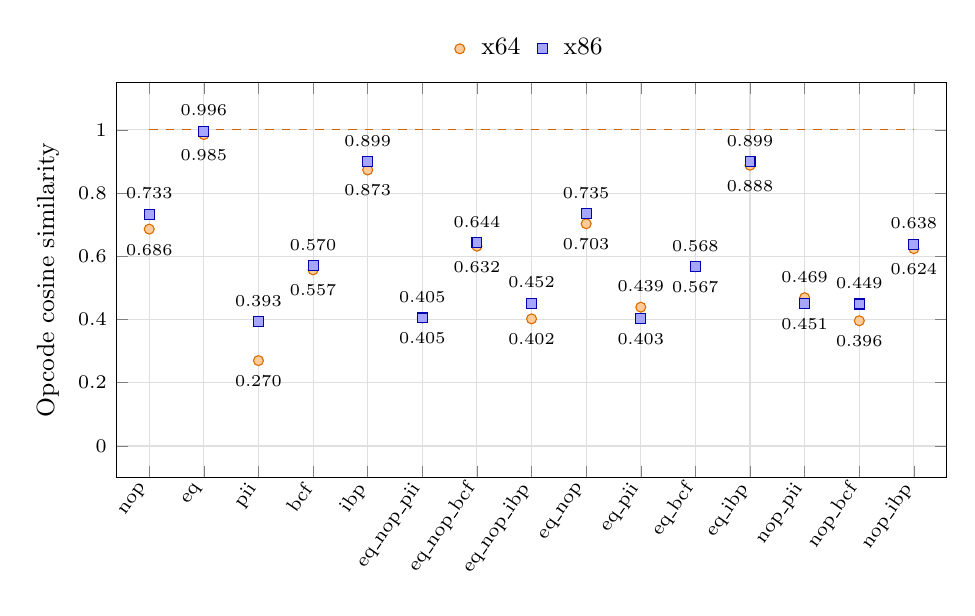
\begin{tikzpicture}
\begin{axis}[
width=\linewidth,height=6.6cm,
ylabel={Opcode cosine similarity},ymin=-0.1,ymax=1.15,xmin=-0.6,xmax=14.6,
xtick={0,...,14},
xticklabels={nop,eq,pii,bcf,ibp,eq\_nop\_pii,eq\_nop\_bcf,eq\_nop\_ibp,eq\_nop,eq\_pii,eq\_bcf,eq\_ibp,nop\_pii,nop\_bcf,nop\_ibp},
xticklabel style={rotate=55,anchor=east,font=\scriptsize},
yticklabel style={font=\scriptsize},label style={font=\small},
grid=major,grid style={gray!25},scaled y ticks=false,
legend style={at={(0.5,1.03)},anchor=south,legend columns=2,column sep=4pt,font=\small,draw=none},
clip=false,
]
\addplot[orange!80!black,dashed,no marks,forget plot] coordinates {(0,1) (14,1)};
\addplot[only marks,mark size=1.8pt,orange!85!black,mark=*,mark options={fill=orange!40}] coordinates {(0,0.686) (1,0.985) (2,0.270) (3,0.557) (4,0.873) (5,0.405) (6,0.632) (7,0.402) (8,0.703) (9,0.439) (10,0.567) (11,0.888) (12,0.469) (13,0.396) (14,0.624)};
\addlegendentry{x64}
\node[anchor=north,yshift=-2pt,font=\fontsize{6}{7}\selectfont] at (axis cs:0,0.686) {0.686};
\node[anchor=north,yshift=-2pt,font=\fontsize{6}{7}\selectfont] at (axis cs:1,0.985) {0.985};
\node[anchor=north,yshift=-2pt,font=\fontsize{6}{7}\selectfont] at (axis cs:2,0.270) {0.270};
\node[anchor=north,yshift=-2pt,font=\fontsize{6}{7}\selectfont] at (axis cs:3,0.557) {0.557};
\node[anchor=north,yshift=-2pt,font=\fontsize{6}{7}\selectfont] at (axis cs:4,0.873) {0.873};
\node[anchor=south,yshift=2pt,font=\fontsize{6}{7}\selectfont] at (axis cs:5,0.405) {0.405};
\node[anchor=north,yshift=-2pt,font=\fontsize{6}{7}\selectfont] at (axis cs:6,0.632) {0.632};
\node[anchor=north,yshift=-2pt,font=\fontsize{6}{7}\selectfont] at (axis cs:7,0.402) {0.402};
\node[anchor=north,yshift=-2pt,font=\fontsize{6}{7}\selectfont] at (axis cs:8,0.703) {0.703};
\node[anchor=south,yshift=2pt,font=\fontsize{6}{7}\selectfont] at (axis cs:9,0.439) {0.439};
\node[anchor=north,yshift=-2pt,font=\fontsize{6}{7}\selectfont] at (axis cs:10,0.567) {0.567};
\node[anchor=north,yshift=-2pt,font=\fontsize{6}{7}\selectfont] at (axis cs:11,0.888) {0.888};
\node[anchor=south,yshift=2pt,font=\fontsize{6}{7}\selectfont] at (axis cs:12,0.469) {0.469};
\node[anchor=north,yshift=-2pt,font=\fontsize{6}{7}\selectfont] at (axis cs:13,0.396) {0.396};
\node[anchor=north,yshift=-2pt,font=\fontsize{6}{7}\selectfont] at (axis cs:14,0.624) {0.624};
\addplot[only marks,mark size=1.8pt,blue!70!black,mark=square*,mark options={fill=blue!35}] coordinates {(0,0.733) (1,0.996) (2,0.393) (3,0.570) (4,0.899) (5,0.405) (6,0.644) (7,0.452) (8,0.735) (9,0.403) (10,0.568) (11,0.899) (12,0.451) (13,0.449) (14,0.638)};
\addlegendentry{x86}
\node[anchor=south,yshift=2pt,font=\fontsize{6}{7}\selectfont] at (axis cs:0,0.733) {0.733};
\node[anchor=south,yshift=2pt,font=\fontsize{6}{7}\selectfont] at (axis cs:1,0.996) {0.996};
\node[anchor=south,yshift=2pt,font=\fontsize{6}{7}\selectfont] at (axis cs:2,0.393) {0.393};
\node[anchor=south,yshift=2pt,font=\fontsize{6}{7}\selectfont] at (axis cs:3,0.570) {0.570};
\node[anchor=south,yshift=2pt,font=\fontsize{6}{7}\selectfont] at (axis cs:4,0.899) {0.899};
\node[anchor=north,yshift=-2pt,font=\fontsize{6}{7}\selectfont] at (axis cs:5,0.405) {0.405};
\node[anchor=south,yshift=2pt,font=\fontsize{6}{7}\selectfont] at (axis cs:6,0.644) {0.644};
\node[anchor=south,yshift=2pt,font=\fontsize{6}{7}\selectfont] at (axis cs:7,0.452) {0.452};
\node[anchor=south,yshift=2pt,font=\fontsize{6}{7}\selectfont] at (axis cs:8,0.735) {0.735};
\node[anchor=north,yshift=-2pt,font=\fontsize{6}{7}\selectfont] at (axis cs:9,0.403) {0.403};
\node[anchor=south,yshift=2pt,font=\fontsize{6}{7}\selectfont] at (axis cs:10,0.568) {0.568};
\node[anchor=south,yshift=2pt,font=\fontsize{6}{7}\selectfont] at (axis cs:11,0.899) {0.899};
\node[anchor=north,yshift=-2pt,font=\fontsize{6}{7}\selectfont] at (axis cs:12,0.451) {0.451};
\node[anchor=south,yshift=2pt,font=\fontsize{6}{7}\selectfont] at (axis cs:13,0.449) {0.449};
\node[anchor=south,yshift=2pt,font=\fontsize{6}{7}\selectfont] at (axis cs:14,0.638) {0.638};
\end{axis}
\end{tikzpicture}
\Description{Cosine similarity between original-corpus and configuration-level opcode-frequency vectors; the reference level is one. Orange circles identify x64 and blue squares identify x86.}
\caption{Cosine similarity between original-corpus and configuration-level opcode-frequency vectors; the reference level is one. Data from Fig.~7 of~\cite{zone_secrypt_2026}; redrawn for the present format.}
\label{fig:cosine_similarity}
\end{figure}

Figure~\ref{fig:cosine_similarity} shows higher similarity for EQ and IBP
than for insertion-heavy configurations. Together with length and entropy,
this characterizes representation changes. Functional preservation is
assessed separately by the execution tests in Section~\ref{sec:results}.

\section{Limitations and Defensive Implications}\label{sec:limitations}
The following limitations concern the original implementation and experiments~\cite{zone_secrypt_2026}. Sections~\ref{sec:code_data}--\ref{sec:wrapping} describe subsequent work motivated by these observations; the residual limits of the added paths are discussed in Section~\ref{sec:extension_limits}.
\begin{itemize}
    \item \textbf{Instruction coverage.} Less common instructions, including the example \texttt{JRCXZ}, can require handling not exercised by this corpus. Testing a fixed collection of 102 inputs does not establish complete x86/x64 coverage.
    \item \textbf{Code--data ambiguity.} Embedded strings may partly decode as instructions. Table~\ref{tab:broken-payload} illustrates an input in which the bytes of \texttt{.exe} are interpreted as a branch. Rewriting the resulting instruction interpretation can corrupt the embedded string.
\end{itemize}

Recovering instructions and references is a general challenge in static
analysis~\cite{staticdisasmTuringComplete}. The two published examples
below show one concrete distinction: an inline string versus a string
encoded within an instruction operand.

\begin{table}[t]
    \caption{Inline-data example affected by rewriting. Reproduced from Table~5 of~\cite{zone_secrypt_2026}.}
    \label{tab:broken-payload}
    \small
    \centering
    \setlength{\tabcolsep}{3pt}
    \begin{tabular}{ll}
        \hline
        \textbf{Bytes}  & \textbf{Instruction} \\ \hline
        \verb|0x109 b'\xff\xd5'|  & call  rbp \\ \hline
        \verb|0x10b b'c'|         & .byte 0x63 \\ \hline
        \verb|0x10c b'a'|         & .byte 0x61 \\ \hline
        \verb|0x10d b'l'|         & insb  byte ptr [rdi], dx \\ \hline
        \verb|0x10e b'c'|         & .byte 0x63 \\ \hline
        \verb|0x10f b'.exe'|      & js    0x178 \\ \hline
        \verb|0x113 b'\x00'|      & .byte 0x00 \\ \hline
    \end{tabular}
\end{table}

In Table~\ref{tab:broken-payload}, part of the trailing
\texttt{calc.exe} string decodes as a branch and can be modified by rewriting.

\begin{table}[t]
    \caption{Immediate-operand example. Reproduced from Table~6 of~\cite{zone_secrypt_2026}.}
    \label{tab:functional-payload}
    \small
    \centering
    \setlength{\tabcolsep}{3pt}
    \begin{tabular}{ll}
        \hline
        \textbf{Bytes}                  & \textbf{Instruction} \\ \hline
        \verb|0x8d b'Q'|              &  push     rcx \\ \hline
        \verb|0x8e b'H\xb9calc.exe'|  &  movabs   rcx, 0x6578652e636c6163 \\ \hline
        \verb|0x98 b'Q'|              &  push     rcx \\ \hline
        \verb|0x99 b'H\x8d\x0c\$'|     & lea      rcx, [rsp] \\ \hline
        \verb|0x9d b'H1\xd2'|          & xor      rdx, rdx \\ \hline
        \verb|0xa0 b'H\xff\xc2'|       & inc      rdx \\ \hline
        \verb|0xa3 b'H\x83\xec('|      & sub      rsp, 0x28 \\ \hline
        \verb|0xa7 b'\xff\xd0'|        & call     rax \\ \hline
    \end{tabular}
\end{table}

In Table~\ref{tab:functional-payload}, the string is an immediate
operand at \texttt{0x8e}; the reported transformation avoids that inline-data
failure. Section~\ref{sec:code_data} develops the corresponding preparation stage.

\subsection{Mitigations and Countermeasures}
Changing the binary representation does not remove a program's observable actions. Defensive analysis can consider memory protections, execution patterns, API activity, and network behavior in addition to static bytes. Recognition of a transformation engine is another possibility: repeated artifacts of a common toolchain can persist across outputs, as documented for Shikata Ga Nai~\cite{sgnstrong}. Statistical or learned detectors must also account for benign programs that share similar features. These are defensive considerations arising from the study, not results of an additional detection experiment.

\section{Comparison with Shikata Ga Nai}\label{sec:comparison}
The conference study~\cite{zone_secrypt_2026} compared Zone with the
Shikata Ga Nai (SGN) polymorphic encoder~\cite{sgnarticle}, using the
original x86 encoder and an unofficial x64 implementation~\cite{sgn64}.
Reported mean static detection rates were 0\% for SGN versus 0.57\% for
Zone on x64, and 10.22\% versus 0.25\% on x86; PII reached 0\% on both.

SGN varies an encoded body and its decoding stub, whose recurring
features may be recognized~\cite{sgnstrong}. The conference study also
scanned memory dumps from SGN execution and reported verdicts matching
the unencoded inputs, consistent with exposure of the original body after
decoding~\cite{codeExtraction}. Zone instead intends to retain the
rewritten representation during execution. The dump comparison concerns
the recognizability of submitted memory contents, within the scope
defined in Section~\ref{sec:introduction}.

% Added material extends the original study retained above.
\section{Code--Data Identification and Data-Preserving Rewriting}
\label{sec:code_data}
\subsection{Why Data Identification Comes Before Transformation}
A raw binary contains no explicit distinction between instructions and
embedded strings or tables. String bytes may decode as plausible
instructions, so rewriting their apparent instruction sequence can corrupt
data. Table~\ref{tab:broken-payload} illustrates this failure; in
Table~\ref{tab:functional-payload}, the string instead occupies an
instruction operand that must remain intact.

Preparation separates two responsibilities. \emph{Identification} proposes
data regions; \emph{data handling} preserves supported objects and updates
their references after layout changes. A reference is an instruction
operand or address calculation pointing to code or data. Preserving a
string is insufficient if the program still reads its old address.
Figure~\ref{fig:extended_pipeline} shows the alternative symbolic/heuristic
and LLM classifiers feeding shared handling. Independently, instructions
can be transformed natively or by an LLM: classification does not imply
LLM transformation.
\begin{figure}[t]
\centering
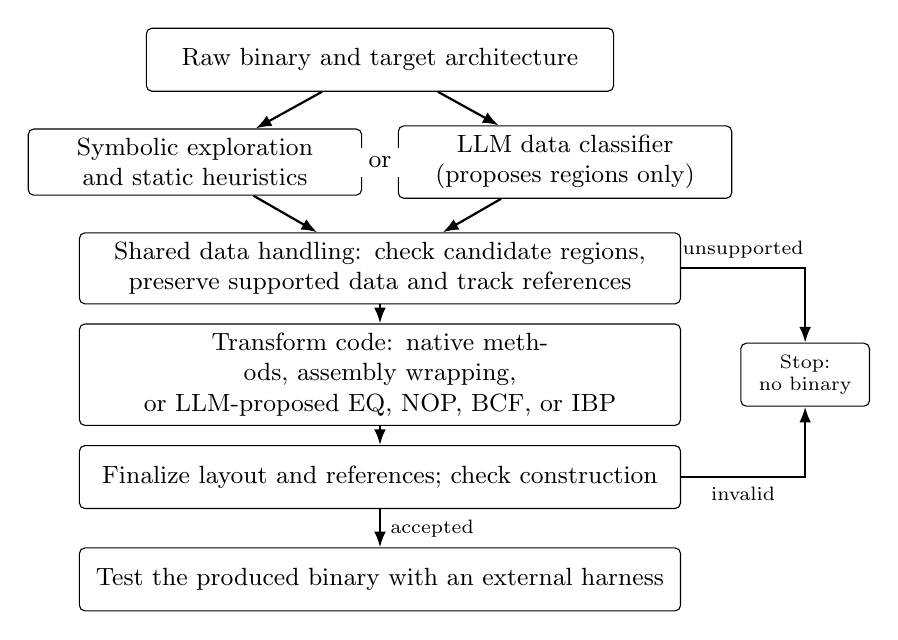
\begin{tikzpicture}[
  box/.style={draw,rounded corners=2pt,align=center,font=\small,
    minimum height=0.8cm,text width=4.0cm},
  arrow/.style={-{Latex[length=2mm]},thick}]
\node[box,text width=5.7cm] (input) at (0,0) {Raw binary and target architecture};
\node[box] (sym) at (-2.35,-1.3) {Symbolic exploration\\and static heuristics};
\node[box] (llm) at (2.35,-1.3) {LLM data classifier\\(proposes regions only)};
\node[box,text width=7.4cm] (data) at (0,-2.65) {Shared data handling: check candidate regions,\\preserve supported data and track references};
\node[box,text width=7.4cm] (trans) at (0,-4.0) {Transform code: native methods, assembly wrapping,\\or LLM-proposed EQ, NOP, BCF, or IBP};
\node[box,text width=7.4cm] (build) at (0,-5.3) {Finalize layout and references; check construction};
\node[box,text width=7.4cm] (test) at (0,-6.6) {Test the produced binary with an external harness};
\node[box,text width=1.4cm,font=\scriptsize] (stop) at (5.4,-4.0) {Stop:\\no binary};
\draw[arrow] (input) -- (sym);
\draw[arrow] (input) -- (llm);
\draw[arrow] (sym) -- (data);
\draw[arrow] (llm) -- (data);
\draw[arrow] (data) -- (trans);
\draw[arrow] (trans) -- (build);
\draw[arrow] (build) -- node[right,font=\scriptsize] {accepted} (test);
\draw[arrow] (data.east) -- node[above,font=\scriptsize] {unsupported} (5.4,-2.65) -- (stop.north);
\draw[arrow] (build.east) -- node[below,font=\scriptsize] {invalid} (5.4,-5.3) -- (stop.south);
\node[font=\small,fill=white] at (0,-1.3) {or};
\end{tikzpicture}
\caption{Organization of the extensions. Identification proposes data
regions; shared handling and construction checks determine whether a
binary reaches the independent functional test.}
\label{fig:extended_pipeline}
\end{figure}

\subsection{What a Classification Result Means}
For an input of $n$ bytes, a proposed data region is an interval $[s,e)$:
it starts at offset $s$ from the beginning of the input and includes every
byte up to, but not including, $e$. For example, $[2,8)$ denotes six bytes.
An optional type describes a string encoding, such as ASCII or UTF-16LE,
or another data object. The output is a set of candidate intervals,
not a replacement binary.

Three stages must be distinguished: a classifier's proposed regions,
regions accepted by the engine's checks, and regions actually extracted
from the instruction stream. A correct proposal may still be unsupported
if its references cannot be updated. Conversely, different proposals can
produce the same binary when the shared checks retain the same objects.
The experiments compare annotations, accepted outputs, and final hashes
at their respective stages.

\subsection{Symbolic Exploration Combined with Static Heuristics}
The non-LLM method combines three sources of evidence. First, static
analysis recovers a control-flow graph (CFG): nodes represent basic blocks
of instructions and edges represent possible transfers of execution.
Zone uses angr's CFGFast analysis for this initial structure~\cite{angr_cfg_docs}.
Second, symbolic execution explores possible paths while representing
unknown register and memory values as symbolic expressions. This supplies
additional evidence about which instructions can be reached. Third,
pattern-based rules recognize printable ASCII and UTF-16LE string
candidates, including their terminators, and consider regions identified
as data by the control-flow analysis. Candidates overlapping confirmed
instruction bytes are filtered out. These rules supply recognizable
patterns and supporting evidence; an unexplored region alone is not
sufficient to classify it as data.

An observed instruction protects its entire decoded byte span, not only
its starting address. This matters for variable-length instructions: an
interior byte should not become a data candidate merely because the
explorer recorded only the instruction's first byte. Newly observed entry
points can also support another graph-recovery pass. Printable candidates
that overlap observed code are excluded by the string heuristic; candidates
overlapping graph-recovered code need additional structural support.

Exploration is bounded by time, solver, and state limits. The initial state
does not reproduce every feature of a Windows process, including all
external API behavior. Consequently, an unvisited region is \emph{unknown},
not proven to be data. Reports retain the evidence category, stopping
reason, unresolved states, and errors. These distinctions prevent a
partial execution search from being presented as a complete partition of
the binary into code and data.

\subsection{LLM Identification and Shared Data Handling}
The LLM receives hexadecimal bytes, a linear disassembly, and candidate
printable strings, and returns structured data intervals. The disassembly
is evidence to assess, not a trusted annotation. This mode neither
extracts data nor rewrites instructions.

Deterministic parsing rejects empty or out-of-bounds intervals and invalid
overlaps. The engine examines supported references and retains accepted
data separately from the instructions. After transformation, it finalizes
references using the new layout. Integrity checks compare retained bytes
with their saved originals at the final locations and verify supported
references against their expected destinations; mismatches reject the
construction. Address handling is architecture-specific.

For example, a benign routine may copy embedded strings \texttt{alpha}
and \texttt{beta} into a buffer. Identification locates the strings;
handling preserves their contents and links; the final execution test
checks the expected buffer. These test different stages of the pipeline.

Correction requests append the rejected answer and validator diagnostic
to the conversation and ask for a revised proposal, within the configured
attempt limit. An interval beyond the input, for example, receives an
out-of-bounds diagnostic. Classification feedback concerns data locations;
transformation feedback concerns assembly. Likewise, examples illustrating
classification are independent of the transformation zero-shot/two-shot
conditions in the next section.

Symbolic identification can reuse cached regions for an input; references
are recomputed for the working representation. This preparation cache
does not replace LLM requests: the classification benchmark records
18 actual API calls, while repeated morphing requests can share preparation
but generate new instruction listings. Both classifiers feed the same
handling, which can reconcile different proposals into identical binaries.

\section{LLM-Assisted Assembly Transformation}\label{sec:llm}
\subsection{What the Model Is Asked to Change}
In this mode the LLM receives assembly and proposes a new instruction
sequence intended to preserve behavior. It supports the EQ, NOP, BCF,
and IBP families introduced in Section~\ref{sec:background}; data
classification instead returns only locations. PII and wrapping remain
native operations because their layout and encoding constraints are not
implemented in the LLM interface's requests and validators. This is an
implementation boundary, not an intrinsic limitation of language models.

Zone prepares an assembly listing with identified data retained separately;
identification itself may use an LLM. Symbolic labels identify locations
independently of changing byte offsets. The model returns a complete listing,
which Zone assembles, restores with the retained data, and validates.
Keeping exact data bytes outside generation avoids requiring the model to
reproduce unchanged content and separates instruction rewriting from data
preservation. An end-to-end alternative is not evaluated. The original binary, prepared listing, and final
binary are different representations: internal LLM similarity compares
prepared and returned listings, excluding changes made during preparation.

The requested model is \texttt{deepseek-flash}. Provider documentation
accessed on 15 November 2026 maps this alias to DeepSeek-V4.1-Flash~\cite{deepseek_models}.
The experiment records retain the alias, not an independently verified
provider snapshot for each call.
Both LLM roles request temperature 0.2, with no sampling seed or explicit
top-p. Repeated requests are not treated as deterministic reproductions.

\subsection{Prompting Conditions and Repeated Attempts}
A system message defines the task, preservation priority, and response
format. The user prompt specifies the architecture, technique-specific
rules, common constraints on machine state, control flow and data,
input-specific notes, and the prepared listing. Uncertain transformations
must remain unapplied; the response must contain only a complete assembly
listing. Both conditions share this structured specification:
\emph{zero-shot} supplies no example, whereas \emph{two-shot} adds two
illustrative input--output examples for the selected technique. The comparison
therefore isolates the addition of demonstrations to the prompt. Shots count
examples, not attempts. Each input, technique, and shot setting defines a
\emph{cell}.

Validation feedback returns a rejected answer and its diagnostic---for
example, a missing label or assembly failure---and requests a correction.
It contains neither a functional success signal nor a scanner verdict.
The controlled benchmark disables correction and makes three independent
single-generation requests per cell, retaining failures. The original-corpus
campaign targets one output per cell, with some retries and failed
restarts in its logs. Its results are cell outcomes rather than uniform
first-generation success rates (Section~\ref{sec:methodology}).

\subsection{From a Proposed Listing to an Assessed Output}
Validation checks whether the response can be assembled and decoded,
whether tracked control-flow targets remain consistent, whether preserved
data survives, and whether the requested transformation's structural
requirements are met. A response can fail at any of these stages, or be
truncated before it contains a complete listing. Passing them means that
Zone accepts a constructed output, which then proceeds to the execution test.

An external \emph{test harness} launches the output and records its result.
It compares the complete expected buffer for controlled programs and
checks the class-specific observable for original payloads
(Section~\ref{sec:methodology}).


Saved records distinguish requests, accepted outputs, subsequent execution
results, time, and estimated cost.

\section{Assembly Wrapping: Mechanism and Integration}\label{sec:wrapping}
\subsection{Reading the Same Bytes from Different Starting Points}
Assembly wrapping relies on a property of x86 and x64: instructions have
variable lengths, and the starting byte determines how a decoder groups
the following bytes into instructions. The same stored bytes can therefore
have two interpretations when read from different starting points.

Consider two views of one region. In the \emph{outer view}, a decoder sees
an instruction followed by its immediate operand, a constant stored inside
that instruction. In the \emph{execution view}, part of that constant's
byte field is read as an instruction sequence. The established wrapping
technique uses this overlap to give the stored representation an outer
instruction structure while retaining an intended executable interpretation
within it~\cite{assembly_wrapping}.

Figure~\ref{fig:wrapping_views} shows these two readings of one byte field.
The term \emph{container} refers to the outer instruction; \emph{embedded
sequence} refers to the instructions represented inside its operand bytes.
These are two readings of shared bytes, rather than two copies of the
program. No decryption step is required to obtain the embedded interpretation.

\begin{figure}[t]
\centering
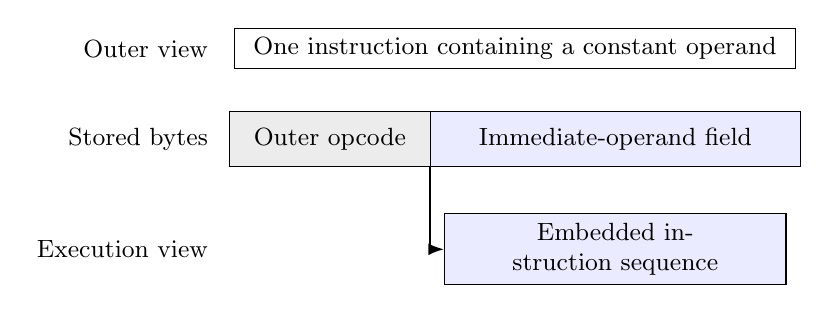
\begin{tikzpicture}[font=\small]
\node[anchor=east] at (0,0.5) {Stored bytes};
\draw[fill=gray!15] (0.15,0.15) rectangle (2.7,0.85);
\draw[fill=blue!8] (2.7,0.15) rectangle (7.4,0.85);
\node at (1.425,0.5) {Outer opcode};
\node at (5.05,0.5) {Immediate-operand field};
\node[anchor=east] at (0,1.65) {Outer view};
\node[draw,align=center,text width=6.9cm] at (3.775,1.65)
  {One instruction containing a constant operand};
\node[anchor=east] at (0,-0.9) {Execution view};
\node[draw,fill=blue!8,align=center,text width=4.1cm] (inside)
  at (5.05,-0.9) {Embedded instruction sequence};
\draw[-{Latex[length=2mm]},thick] (2.7,0.15) -- (2.7,-0.9) -- (inside.west);
\end{tikzpicture}
\caption{Conceptual views of a wrapped region. Starting at the outer
opcode interprets the operand as a constant; entering the embedded
sequence interprets some of those same bytes as instructions.
The drawing is not to scale and omits inter-region control transfers.}
\label{fig:wrapping_views}
\end{figure}

\subsection{What Zone Adds and What the Transformation Requires}
The contribution of this work is the integration and assessment of an
existing technique, with implementations for both architectures. Zone
starts from a prepared instruction stream, groups supported instructions
into wrapped regions, preserves the required execution relationships, and
updates the supported location-dependent references after layout. Some
instructions or local layouts cannot be placed in the main container
representation. For example, an instruction sequence longer than the
available operand field does not fit inside that container. The
implementation retains unsupported cases in ordinary, unwrapped regions. An output may therefore contain both wrapped and ordinary code.

The x86 and x64 implementations share this purpose but use different
encodings and addressing rules. In particular, the available immediate
operand has a different width, affecting which instruction groups fit.
Both architectures are included in the functional evaluation.

\subsection{How Wrapping Is Evaluated}
The evaluation follows three stages: construction of a binary, execution
of its functional test, and static scanning of the produced file.
Construction rate measures how many requested variants are available;
working rate measures how many perform the expected task; detection rate
describes the scanner responses. The full experiment uses all 102 original
payloads, with the same stages reported separately for x64 and x86.

\section{Experimental Design for the Extensions}\label{sec:methodology}
\subsection{What Is Tested, and on Which Programs?}
The evaluation separates three practical questions: whether Zone identifies
embedded data correctly, whether a transformed program still performs its
expected task, and how often static scanners flag the resulting file.
Table~\ref{tab:test_populations} summarizes the inputs used for each question.

\begin{table}[t]
\caption{Test populations. The 13 controlled programs and the 13
selected x64 payloads are different sets with different purposes.}
\label{tab:test_populations}
\centering\small
\begin{tabularx}{\linewidth}{@{}l r Y@{}}
\toprule
Population & Inputs & Purpose \\
\midrule
Controlled functional programs & 13 & Check exact expected output after transformation. \\
Annotated classification programs & 6 & Check which bytes are identified as data. \\
Original Windows payload corpus & 102 & Measure construction, functionality, and static detection. \\
Recovery subset of that corpus & 49 & Compare historical and updated working rates on previously problematic inputs. \\
Data-handling subset of that corpus & 19 & Compare symbolic and LLM identification within the same pipeline. \\
\bottomrule
\end{tabularx}
\end{table}

The 13 \emph{controlled functional programs} (test fixtures) are purpose-built
assembly programs of 19--68 bytes. Six per architecture cover arithmetic,
branches, loops, local calls, combined control flow, and embedded strings;
one extra x64 case accesses data through a computed code address. Each
writes a known result into a 256-byte buffer. A native C runner compares
the entire buffer, including untouched positions, with the expected bytes.
All 13 originals pass.

The six \emph{annotated classification programs} instead test data
locations: two contain multiple strings, one a binary table, two no
separate data, and one instruction bytes resembling text. Correct regions
are annotated before either classifier runs and withheld from the model.
These suites check individual mechanisms; original payloads provide the
broader application-level evaluation.

The original corpus contains 38 x64 and 64 x86 Windows payloads.
Functional tests check the expected dialog, network connection event,
or clean termination for the relevant payload class. All 102 originals pass.
Historical and extended outcomes use the definition of \emph{working}
given in Section~\ref{sec:introduction}.

The recovery comparison selects the 49 original inputs whose historical
working rate was below 50\%: 13 x64 and 36 x86. It compares the same
inputs and 15 transformation configurations before and after the
pipeline update. New results use ten variants per x64 input/configuration
and five per x86 input/configuration. Data-preparation-only controls are
reported separately. The comparison measures the updated pipeline as a
whole, including the improved MessageBox test; it is not an ablation of
data identification alone.

\subsection{Configurations, Repetitions, and Model Calls}
A \emph{cell} combines an input, transformation, and prompting condition:
for example, one x64 program transformed with EQ and two examples.
Repeating that combination gives repetitions of the same cell.

Both LLM roles request temperature 0.2 without a sampling seed or top-p;
these client settings do not imply identical repeated answers.

The native controlled benchmark uses three runs per input and transformation
family. The LLM benchmark uses four families, two prompting conditions,
and three separate single-generation requests per cell. This gives
$7\times4\times2\times3=168$ x64 requests and
$6\times4\times2\times3=144$ x86 requests. All rejected responses and
transport failures remain in the counts. The classification benchmark uses
three LLM requests and one symbolic analysis per annotated program.

On the full original corpus, wrapping uses three randomization seeds per
input, giving $102\times3=306$ planned variants. The LLM experiment has
$102\times4\times2=816$ cells and an output-token limit of 65,536.
It targets one accepted output per cell; two successful cells required a
second generation, and fourteen failed cells were restarted without success.
These results describe the completed campaign, including those retries.
The exploratory prompting comparison pairs outcomes by input and family;
an input-level sensitivity check retains all four families together
(Supplementary Material S1).

The data-handling comparison uses 19 original inputs (13 x64,
six x86) with data extracted by symbolic preparation. Each method proposes
data regions, after which the same deterministic handling and functional
test are applied. Input selection and shared processing are thus held
explicit in interpreting the comparison.

The accompanying artifact records engine versions and request histories.
Native x86 IBP was tested with an earlier implementation than the later
x86 LLM and wrapping experiments; these are separately identified in the
artifact. The native x86 IBP result therefore characterizes that recorded
version; no current-version retest is available, and no version-improvement
claim is inferred from comparing these campaigns.

\subsection{Build Rate, Working Rate, and Classification Accuracy}
Let $N$ be planned cases, $B$ produced binaries, and $W$ binaries passing
the functional test. Build rate is $B/N$, overall working rate is $W/N$,
and working rate among produced binaries is $W/B$.
For example, ten planned cases, eight produced binaries, and six successful
tests give 80\%, 60\%, and 75\%, respectively. The selected-cohort comparison divides
successful tests by recorded tests, matching the available historical
records. The overall update in Table~\ref{tab:overall_working_update}
combines the new rates for retested inputs with the retained historical
rates for other inputs. Each input keeps its historical test-count weight.
This avoids changing the composition of the x86 average merely because
the new campaign uses fewer repetitions. No missing historical outcome is
imputed. The final table row is the arithmetic mean of the 15
configuration rates, not weighted by their sample counts. Detailed
contributions are supplied in Supplementary Material S1. Repeated
executions of one binary are not new variants.

For classification, predicted positions $P$ are bytes labelled as data;
reference positions $G$ are the preannotated correct data bytes. Precision
is $|P\cap G|/|P|$ and recall is $|P\cap G|/|G|$. For a reference string
at bytes 20--29, predicting 20--27 gives 100\% precision and 80\% recall.
Exact matching requires all intervals to agree; programs without separate
data require an empty set. For unannotated original payloads, the evaluation
reports agreement between methods and downstream functionality.

\subsection{Similarity, Detection Rate, Diversity, and Cost}
\paragraph{Representation measurements.}
Historical cosine and entropy definitions are retained. The LLM client's
SequenceMatcher compares prepared and returned listings, filtering
NOP-like operations in the NOP condition. This diagnostic is supplied in
the supplementary records rather than substituted for the historical metrics.

\paragraph{Detection rate.}
We use the same engine-level definition as the historical evaluation:
$d_i=m_i/a_i$, where $m_i$ is the number of malicious responses for file
$i$ and $a_i$ is its total reported engine-response count. Tables report
$\overline d$, the mean across files, as a percentage. For example,
3 malicious responses among 75 give a detection rate of 4\%.
Nonempty current reports contain 75 responses. Unsupported formats,
timeouts, and failed analyses remain in that denominator, consistently
with the historical convention; their breakdown and report-completeness
checks are included in the supplementary records. Missing reports are not
assigned a zero detection rate. Each distinct output hash is scanned once.

\paragraph{Diversity and resources.}
$U$ counts distinct output SHA-256 hashes: identical output bytes count
once for diversity and scanning, even when produced by multiple runs.
A shared hash retains membership in every relevant experimental condition.
Consequently, per-condition unique counts need not sum to the global count.
Time is the recorded duration of a run, including local processing.
Estimated API costs include failed calls and restarted runs. Source records,
version mappings, and the detailed accounting are supplied with the artifact.

\section{Results of the Extended Evaluation}\label{sec:extended_results}
The experiments assess data identification, controlled transformation
behavior, wrapping and LLM transformation on the original corpus, and
recovery of previously failing inputs. Each retains its own input set.

\subsection{Data Identification: Known Answers and Original Payloads}
On the six classification fixtures, all 18 LLM invocations and all
six symbolic runs return the exact reference interval sets
(Table~\ref{tab:new_classifier}). Both methods miss zero data bytes and
classify zero code bytes as data. The three fixtures containing data have
precision and recall equal to one; the other three correctly return no
data. All resulting executions pass their buffer checks. This includes
the deliberately misleading printable-code case, which is rejected as
data rather than extracted as a string.


\begin{table}[t]
\caption{Six programs with independently annotated data locations. $D$ is annotated data bytes.
Exact interval sets are compared against predeclared references.
Mean times are per run in seconds.}
\label{tab:new_classifier}
\centering\small\setlength{\tabcolsep}{4pt}
\begin{tabular}{@{}llrrrrr@{}}
\toprule
Arch. & Case & $D$ & LLM exact & Symbolic exact & LLM time & Sym. time \\
\midrule
x64 & databait & 0 & 3/3 & 1/1 & 4.6 & 2.4 \\
x64 & multidata & 11 & 3/3 & 1/1 & 4.2 & 2.6 \\
x64 & nodata & 0 & 3/3 & 1/1 & 2.1 & 2.4 \\
x64 & table & 16 & 3/3 & 1/1 & 2.6 & 2.4 \\
x86 & multidata & 11 & 3/3 & 1/1 & 4.4 & 2.5 \\
x86 & nodata & 0 & 3/3 & 1/1 & 1.9 & 2.3 \\
\bottomrule
\end{tabular}
\end{table}


On the 19 original data-handling inputs, both pipelines build 19/19
outputs and pass 17/19 checks. Their intervals agree in 9/19 cases and
their final binaries in 16/19: shared handling can reconcile different
proposals. These measure agreement; the annotated tests above measure
classification accuracy. The x86 custom and Meterpreter WinHTTP failures
have identical final binaries under both methods, so these failures do not
distinguish the classifiers. Their root cause is not established here.
On three x64 WinHTTPS inputs, the LLM proposes larger data regions and
produces different, working binaries. Thus, interval disagreement need not
imply functional failure; passing the test does not establish which
classification is more accurate.

The recorded median durations are 123.95 seconds for symbolic preparation
and 59.88 seconds for the LLM arm. The latter's estimated cost is \$0.2218
over 19 runs. These are measured run durations; preparation and caching differ
between the two arms. On the separate six-fixture benchmark,
the total LLM cost is approximately \$0.0059. 

\subsection{Functional Tests on 13 Controlled Programs}
Each native configuration has three tests per input: 21 on the 7 x64
programs and 18 on the 6 x86 programs. Table~\ref{tab:controlled_functional}
reports successful/planned tests and combines the LLM prompting conditions;
separate outcomes are supplied in the supplement.

\begin{table}[t]
\caption{Functional success on the controlled programs. Each entry is
successful tests/planned tests. LLM columns combine zero-shot and two-shot
requests at temperature 0.2. PII is outside this benchmark; wrapping is
native-only. The native x86 IBP row refers to the recorded earlier version.}
\label{tab:controlled_functional}
\centering\small\setlength{\tabcolsep}{7pt}
\begin{tabular}{@{}lrrrr@{}}
\toprule
 & \multicolumn{2}{c}{Native} & \multicolumn{2}{c}{LLM} \\
\cmidrule(lr){2-3}\cmidrule(lr){4-5}
Family & x64 & x86 & x64 & x86 \\
\midrule
EQ & 21/21 & 18/18 & 42/42 & 36/36 \\
NOP & 21/21 & 18/18 & 42/42 & 36/36 \\
BCF & 21/21 & 18/18 & 42/42 & 36/36 \\
IBP & 21/21 & 0/18 & 41/42 & 30/36 \\
Wrapping & 21/21 & 18/18 & -- & -- \\
\bottomrule
\end{tabular}
\end{table}

All native x64 tests pass. Native x86 EQ, NOP, BCF, and wrapping also
pass; the recorded native x86 IBP configuration produces 17 binaries from
18 attempts, but none passes the complete-buffer test.

The LLM produces 305 accepted outputs from 312 requests (97.8\%), and
every accepted output has the correct buffer. The remaining seven requests
comprise five structural-validation rejections and two transport errors.
Thus the main result is functional preservation for all accepted outputs
on these controlled inputs, with construction availability recorded separately.

Repeated output hashes are most visible in EQ. These inputs are short,
offer few locations for substitutions, and are subject to the restricted
set of supported transformations. This provides a straightforward
explanation for limited diversity on this suite; different requests need
not produce different accepted instruction sequences. Detailed hashes,
per-shot outcomes, time, and cost remain available in the supplement.

\subsection{Wrapping on All 102 Original Payloads}
The full-corpus campaign attempts 306 variants, three per input. It constructs
243 binaries (79.4\% of planned cases), of which 170 pass the harness.
Thus $W/N=55.6$\%, whereas $W/B=70.0$\%. These rates report both availability of a transformed binary and
its functional outcome.


\begin{table}[t]
\caption{Wrapping on all 102 original payloads, with three seeds per input.
$U$ counts distinct constructed hashes.}
\label{tab:new_wrap_full}
\centering\small
\begin{tabular}{@{}lrrrrr@{}}
\toprule
Arch. & Inputs & $B/N$ & $W/N$ & $W/B$ & $U$ \\
\midrule
x64 & 38 & 63/114 & 63/114 & 63/63 & 63 \\
x86 & 64 & 180/192 & 107/192 & 107/180 & 144 \\
\bottomrule
\end{tabular}
\end{table}


The two architectures fail at different stages. On x64, 51 attempts do
not build, while all 63 constructed outputs pass. On x86, only twelve
attempts do not build, but 73 of the 180 constructed outputs fail the
harness. All 73 also fail the saved isolated retests; those retests are
not counted as additional variants. There are 207 distinct hashes among
the 243 binaries, showing that different seeds do not always produce
different bytes.

The construction logs include incomplete instruction interpretation and
inconsistent address references. These failure stages have a direct
relationship to preparation: interpreting embedded data as instructions
can prevent a complete valid disassembly, and a reference that no longer
points to the intended location fails the consistency check after layout
changes. The logs identify these symptoms; they do not assign one common
cause to every failed execution.

\subsection{Completed LLM Transformation on the Original Corpus}
All 816 planned cells have an outcome. The campaign constructs 350
outputs, and 275 pass the external harness: a build rate of 42.9\%, an
overall working rate of 33.7\%, and a working rate among builds of 78.6\%.
Table~\ref{tab:payload_llm} shows the complete architecture/family/shot
breakdown. These are pipeline outcomes, including the retries described
in Section~\ref{sec:methodology}.


\begin{table}[t]
\caption{LLM transformation of all 102 original payloads. $N$: planned cells; $B$: accepted
builds; $W$: builds passing the external harness; $U$: distinct built-output
hashes within the condition. Every planned cell is retained.}
\label{tab:payload_llm}
\centering\small
\begin{tabular}{@{}lllrrrr@{}}
\toprule
Arch. & Family & Shots & $N$ & $B$ & $W$ & $U$ \\
\midrule
x64 & EQ & 0 & 38 & 7 & 7 & 7 \\
x64 & EQ & 2 & 38 & 6 & 6 & 6 \\
x64 & NOP & 0 & 38 & 8 & 8 & 8 \\
x64 & NOP & 2 & 38 & 6 & 6 & 6 \\
x64 & BCF & 0 & 38 & 6 & 6 & 6 \\
x64 & BCF & 2 & 38 & 6 & 5 & 6 \\
x64 & IBP & 0 & 38 & 6 & 6 & 6 \\
x64 & IBP & 2 & 38 & 8 & 8 & 8 \\
\midrule
x86 & EQ & 0 & 64 & 34 & 25 & 30 \\
x86 & EQ & 2 & 64 & 36 & 28 & 34 \\
x86 & NOP & 0 & 64 & 38 & 28 & 38 \\
x86 & NOP & 2 & 64 & 35 & 27 & 35 \\
x86 & BCF & 0 & 64 & 40 & 31 & 40 \\
x86 & BCF & 2 & 64 & 36 & 26 & 36 \\
x86 & IBP & 0 & 64 & 39 & 28 & 36 \\
x86 & IBP & 2 & 64 & 39 & 30 & 38 \\
\bottomrule
\end{tabular}
\end{table}



On x64, only 53/304 cells produce binaries, but 52/53 of those binaries
pass. On x86, 297/512 produce binaries and 223/297 pass. Construction is
therefore the principal observed bottleneck on x64, while x86 also has a
substantial failure rate after construction. The controlled programs isolate small instruction and data patterns;
the original payloads add larger listings and more complex layouts.
The two experiments therefore measure different levels of difficulty.

Zero-shot produces 178 builds and 139 passing outputs from 408 cells;
two-shot produces 172 builds and 136 passing outputs from 408 cells.
Their overall working rates are 34.1\% and 33.3\%. Among 408 paired
input/family conditions, 21 work only with zero-shot and 18 only with
two-shot (exact two-sided McNemar $p=0.749$). An input-level sign-flip
check, retaining the four families together, gives $p=0.752$. These
exploratory comparisons provide no evidence of an advantage under this
protocol; they do not establish equivalence. Full calculations and
assumptions are supplied in Supplementary Material S1.

The 466 failed cells have recorded error categories comprising 245
disassembly/boundary errors, 74 validation errors, 53 output-length
terminations, one transport error, and 93 other errors. These labels
describe the observed failure stage, not proven root causes. In particular,
truncation means the response reaches its output limit before delivering
a complete acceptable listing; it is distinct from a generated program
failing at execution time.

The 350 built outputs contain 323 distinct hashes. The median retained-run duration is
160.3 seconds, including local processing. Summing the representative
record for each cell gives an estimated \$19.2700, but including the
14 restarted failed runs raises recorded campaign cost to
\$19.6258. The latter is the appropriate total for work actually recorded;
missing usage for one run prevents claiming complete billing coverage.

\subsection{Updated Working Rates by Transformation}
\label{sec:recovery}
The recovery campaign retests 49 previously low-rate inputs: 13 x64 and
36 x86. On this selected subset, the x64 working rate rises from
23/1,941 (1.2\%) to 1,564/1,950 (80.2\%). The x86 rate rises from
772/5,195 (14.9\%) to 699/2,700 (25.9\%). The denominators differ:
5,195 counts available historical tests, generally with ten repetitions;
2,700 comprises $36$ inputs $\times$ $15$ configurations $\times$ $5$
repetitions. The input cohort is unchanged. These observations measure
the updated implementation and test harness together.

Table~\ref{tab:overall_working_update} places the recovery results back
into the overall historical population. For each transformation, the
retested inputs use their updated rates; other inputs retain their
historical rates. Keeping the original input weights prevents fewer x86
repetitions from reducing the influence of difficult inputs.

The reconstructed mean across the 15 configurations increases from
55.6\% to 82.6\% on x64 and from 45.0\% to 50.3\% on x86.
These are summaries of combined historical and updated evidence. Historical and updated rates appear together in the table, with the
reconstruction stated explicitly.

\begin{table}[t]
\caption{Overall working rates (\%): historical measurements and a
reconstructed update using the recovery tests. The update replaces rates
only for the 49 retested inputs and retains historical rates for the rest.
Historical rates are recomputed from the retained test records of~\cite{zone_secrypt_2026}; input weights are held fixed. Within each configuration, input weights are historical test counts.
The final row gives every configuration weight $1/15$, irrespective of
its sample count; it is not a pooled success/test ratio.
This is a combined evidence summary, not a new execution of the full corpus.}
\label{tab:overall_working_update}
\centering\small\setlength{\tabcolsep}{5pt}
\begin{tabular}{@{}lrrrr@{}}
\toprule
 & \multicolumn{2}{c}{x64} & \multicolumn{2}{c}{x86} \\
\cmidrule(lr){2-3}\cmidrule(lr){4-5}
Configuration & Historical & Updated & Historical & Updated \\
\midrule
NOP & 65.5 & 92.1 & 48.3 & 49.1 \\
EQ & 65.5 & 99.7 & 77.5 & 76.2 \\
PII & 60.3 & 89.2 & 38.8 & 43.9 \\
BCF & 65.8 & 94.5 & 52.7 & 66.1 \\
IBP & 65.8 & 94.2 & 51.7 & 57.2 \\
EQ+NOP+PII & 64.2 & 86.3 & 24.0 & 26.9 \\
EQ+NOP+BCF & 1.1 & 29.5 & 43.9 & 54.7 \\
EQ+NOP+IBP & 65.8 & 91.3 & 40.8 & 42.8 \\
NOP+EQ & 66.0 & 90.5 & 48.1 & 49.2 \\
NOP+PII & 57.3 & 80.1 & 29.3 & 32.5 \\
NOP+BCF & 0.3 & 28.8 & 45.8 & 53.3 \\
NOP+IBP & 66.3 & 89.9 & 40.5 & 44.7 \\
EQ+PII & 57.3 & 86.5 & 28.0 & 31.7 \\
EQ+BCF & 66.8 & 92.6 & 55.2 & 67.3 \\
EQ+IBP & 66.0 & 94.4 & 50.6 & 58.4 \\
\midrule
\textbf{Mean} & 55.6 & 82.6 & 45.0 & 50.3 \\
\bottomrule
\end{tabular}
\end{table}


The lower x86 recovery rate concerns a deliberately difficult subset,
not all x86 inputs. Of its 36 inputs, 13 still have no successful
transformed variant. Preparation-only controls pass 340/360 tests (94.4\%),
whereas adding the native transformations yields 699/2,700 (25.9\%).
This separates successful preparation from the additional transformation
failures; it does not support attributing every remaining failure to data
identification. The dominant recorded execution symptom is an access
violation, which alone does not identify the underlying implementation error.

The improvement is substantially stronger on x64. Even excluding
MessageBox, whose test recognition was corrected, the selected x64 rate
rises from 19/1,791 (1.1\%) to 1,414/1,800 (78.6\%). Per-input and
per-configuration counts, including the selected-subset comparison, remain
available in the supplementary records.

\subsection{Overall Detection Rates for Wrapping and LLM Transformation}
The detection evaluation covers the outputs from the full 102-input LLM
campaign, not only the separate 19-input data-identification experiment.
Of the 816 planned LLM cells, 350 produce binaries, representing 323
distinct hashes. Table~\ref{tab:current_scans} reports the mean engine
detection rate using the same definition as the historical paper.

\begin{table}[!htbp]
\caption{Static detection of the current outputs. Files: produced binaries;
hashes: distinct contents; reports: nonempty scan results. DR is the mean
percentage of engine responses marked malicious.
The working-output row is a subset of the overall LLM row. Report
completeness and response-category details are supplied in the supplement.}
\label{tab:current_scans}
\centering\small\setlength{\tabcolsep}{6pt}
\begin{tabular}{@{}lrrrr@{}}
\toprule
Condition & Files & Hashes & Reports & DR (\%) \\
\midrule
Wrapping & 243 & 207 & 207 & 0.00 \\
LLM x64 & 53 & 51 & 51 & 8.86 \\
LLM x86 & 297 & 272 & 271 & 4.35 \\
\midrule
LLM overall & 350 & 323 & 322 & 5.06 \\
LLM working outputs & 275 & 263 & 263 & 5.89 \\
\bottomrule
\end{tabular}
\end{table}

The overall LLM mean detection rate, 5.06\%, corresponds to 3.80 malicious
engine responses per file. The working-output subset has 263 distinct
hashes and a mean rate of 5.89\%, distinguishing functional outputs from
the complete set of constructed binaries.

All 207 wrapping hashes have nonempty reports with no malicious responses.
These static raw-file measurements use the historical engine-response
denominator (Section~\ref{sec:methodology}). Data-identification scans and
earlier pilots are archived separately in the supplementary evidence.


\clearpage
\section{Related Work}\label{sect:related_work}
\paragraph{Metamorphic rewriting and software protection.}
Instruction substitution, insertion, and control-flow changes predate
this work and appear across both offensive and defensive
research~\cite{survey1,survey2}. Earlier engines, including
W95/Regswap~\cite{desai2010highly} and MetaPHOR~\cite{MetaPHOR}, illustrate
register substitution and code reorganization. Studies of highly
metamorphic programs also examine the relationship between the diversity
of generated variants and the regularities that remain available to
detectors~\cite{desai2008towards,desai2010highly,szor2001hunting}.
Zone uses established transformation families within a payload-level
binary rewriting workflow; the contribution is evaluated through the
resulting construction, functional, and detection outcomes.

Compiler-based protection provides a different starting representation.
Obfuscator-LLVM applies transformation passes to LLVM intermediate
representation, with advantages for language and architecture
coverage~\cite{llvmobf}. Zone instead starts from raw machine code without
source or debugging symbols. The relevant distinction is the information
available before transformation: code boundaries and references must be
recovered from the binary. Consequently, findings from a compiler-based
setting do not directly establish reliability for the inputs studied here.
Practical binary-obfuscation work likewise identifies disassembly and
reference handling as central concerns~\cite{bin2binobf}.

\paragraph{LLM-based transformation.}
Madani~\cite{llm2} investigates LLM-driven program mutation and a
self-testing mutation framework, motivating the evaluation of generated
variants alongside their proposed changes. Mohseni et al.~\cite{llmobf}
introduce MetamorphASM and its MAD dataset of 328,200 assembly samples,
covering dead-code insertion, register substitution, and control-flow
changes. Their study compares multiple language models using
information-theoretic measurements and human review.

Our evaluation addresses a complementary question: how often an LLM
proposal can pass the complete path from prepared assembly to a
constructed binary and an observed functional outcome. It distinguishes
two LLM roles, data identification and instruction transformation, and
compares zero-shot and two-shot requests on a fixed input corpus.
The controlled programs provide known outputs, while the original
payloads exercise larger and more varied layouts. These experimental
populations and endpoints differ from MAD; their success rates should
therefore be read within their respective protocols rather than as a
direct ranking of the systems.

\paragraph{Analysis and detection.}
Metamorphic detection studies include Hidden Markov
Models~\cite{wong2006hunting,desai2010highly}, static comparison of
program semantics~\cite{identifyingmeth}, and genetic-algorithm-based
methods~\cite{methgenetic}. Encoding introduces another representation
change: investigations of SGN examine recognizable properties of its
decoder~\cite{sgnstrong}, while CodeXt studies recovery of hidden attack
code from memory dumps through selective symbolic
execution~\cite{codeExtraction}. These works motivate distinguishing
static file measurements from observations of execution and memory.
The scan results reported here characterize submitted raw files; the
functional tests answer a separate question about the preserved behavior.

\paragraph{Relationship to the original Zone paper.}
Our conference article introduced the PII design and evaluated native
transformations on 102 Windows payloads~\cite{zone_secrypt_2026}. The
present article extends that study with code--data identification,
LLM-assisted transformation, and assembly-wrapping integration.
Bounded symbolic and static analysis inform the data-preparation
stage~\cite{angr_cfg_docs}; assembly wrapping follows its existing
description and antecedents in overlapping
instructions~\cite{assembly_wrapping}. The added contribution is the
integration and evaluation of these paths, including the recovery study,
controlled tests, and completed original-corpus campaigns.

\section{Conclusions and Future Work}\label{sec:conclusion3}\label{sec:extension_limits}
We have extended our SECRYPT 2026 study of Zone~\cite{zone_secrypt_2026}
from its original native transformations to a broader evaluation of
binary rewriting. The extension makes code--data identification and
supported reference handling explicit, separates the LLM roles of
classification and instruction transformation, and integrates the
existing assembly-wrapping technique on x64 and x86. These additions
address the preparation and evaluation of transformed programs alongside
the transformation itself.

The recovery results demonstrate a substantial improvement on inputs
that were difficult for the earlier pipeline. Working rate rises from
1.2\% to 80.2\% on the selected x64 cohort and from 14.9\% to 25.9\% on
x86. Replacing the retested inputs' rates while retaining historical
weights gives mean configuration rates of 82.6\% and 50.3\%, compared
with 55.6\% and 45.0\% historically. This combined summary places the
recovery results in the wider corpus; it does not represent a fresh
execution of every historical test. The gain is larger on x64, while
the residual x86 cases show that the improvement is architecture- and
input-dependent.

The controlled suites and original payloads provide complementary
evidence. Six annotated programs give known answers for data
identification, and 13 functional programs isolate individual programming
patterns. Their small, simple layouts explain why their high success
rates do not automatically extend to the larger corpus. On the 19
original data-handling inputs, symbolic and LLM proposals yield identical
final binaries in 16 cases and the same 17 successful functional outcomes.
This agreement shows that different intermediate proposals can lead to
the same accepted output under shared handling. It also keeps the
classifier's contribution distinct from that of the downstream pipeline.

The full-corpus campaigns expose the difference between producing a
binary and obtaining a working variant. Wrapping constructs 243 binaries
from 306 planned cases, of which 170 pass their functional tests. Every
constructed x64 wrapping output passes, whereas x86 functionality remains
partial. LLM transformation constructs 350 binaries across 816 conditions,
with 275 successful functional outcomes. These results identify
construction failures as a substantial part of the measured outcome;
reporting only accepted outputs would conceal that part of the process.
The recorded native x86 IBP result remains tied to its tested engine
version, separately from these later campaigns.

Zero-shot and two-shot prompting produce similar aggregate outcomes in
this experiment. The evidence supports no consistent advantage for the
additional examples under the tested settings. Static scans report no
malicious responses for the 207 distinct wrapping outputs and a mean
engine detection rate of 5.06\% across 322 nonempty LLM-output reports.
These observations describe the submitted raw files and complement the
functional results. Overall, the extension demonstrates improved
functional reliability and provides a more complete account of the
added transformation paths by reporting construction, execution,
diversity, and detection together.

\subsection{Future Work}\label{sec:future_work}
The main direction for future work is to revisit support for complete
Windows Portable Executable (PE) files. This extension would broaden
the range of programs that Zone can be tested on, enabling experiments
with full applications and more representative execution environments.
It would also help establish the tool's practical applicability: whether
transformed programs continue to load, complete their intended tasks,
and behave consistently under ordinary use. A dedicated study on
documented benign applications of different sizes and build settings
could assess how far the present payload-level findings carry over to
complete software. Functional reliability, processing time, and output
growth would provide complementary measures of practical utility.

A second direction is broader functional validation. Larger controlled
suites and independently annotated code--data examples would extend
coverage of program structures and provide stronger reference outcomes.
Comparisons using the same engine version and test conditions would
help distinguish implementation changes from differences in the inputs.
For LLM-assisted paths, repeated requests with recorded provider versions
and request settings would allow variability to be measured explicitly.
Together, these studies would strengthen the evidence for generalization
and clarify the conditions under which Zone can be used reliably in
practical software-analysis workflows.


\begin{credits}
\subsubsection{\ackname}
This work was partially funded by the University of Perugia's project ``Fighting Cybercrime with OSINT'' (FICO), Civil Safety and Security for Society (WP2).

\subsubsection{\discintname}
The authors have no competing interests to declare.

\subsubsection{Data and Artifact Availability.}
The Zone source repository is available at
\url{https://github.com/jakydibe/Zone}. Supplementary Material S1 contains
the numerical evidence for this article: configuration summaries,
per-cell and per-input outcomes, scan summaries, version provenance,
calculation notes, and checksums. It is supplied as a separate archive
with the manuscript; the public repository is not a frozen snapshot of
all experimental versions. The supplementary archive contains analysis
records, not executable payloads.

\end{credits}

\bibliographystyle{splncs04}
\bibliography{bibliography}
\end{document}
